% LaTeX Template for Project Report, Version 2.0
% (Abstracted from a Major Project Report at CSED, NIT Calicut but can be
% modified easily to use for other reports also.)
%
% Released under Creative Commons Attribution license (CC-BY)
% Info: http://creativecommons.org/licenses/by/3.0/
%
% Created by: Kartik Singhal
% BTech CSE Batch of 2009-13
% NIT Calicut
% Contact Info: kartiksinghal@gmail.com
%
% It is advisable to learn the basics of LaTeX before using this template.
% A good resource to start with is http://en.wikibooks.org/wiki/LaTeX/
%
% All template fields are marked with a pair of angular brackets e.g. <title here>
% except for the ones defining citation names in ref.tex.
%
% Empty space after chapter/section/subsection titles can be used to insert text.
%
% Just compile this file using pdflatex after making all required changes.

\documentclass[12pt, a4paper]{report}

\usepackage[left=1in, right=1in, top=1in, bottom=1in, bindingoffset=5mm]{geometry}
\usepackage[pdftex]{graphicx} %for embedding images
\usepackage{url} %for proper url entries
\usepackage{tabu}
\usepackage[bookmarks, colorlinks=false, pdfborder={0 0 0}, pdftitle={<pdf title here>}, pdfauthor={<author's name here>}, pdfsubject={<subject here>}, pdfkeywords={<keywords here>}]{hyperref} %for creating links in the pdf version and other additional pdf attributes, no effect on the printed document
%\usepackage[final]{pdfpages} %for embedding another pdf, remove if not required
\usepackage{etoolbox}% http://ctan.org/pkg/etoolbox
\makeatletter
\patchcmd{\@makechapterhead}{\vspace*{50\p@}}{}{}{}% Removes space above \chapter head
\patchcmd{\@makeschapterhead}{\vspace*{50\p@}}{}{}{}% Removes space above \chapter* head
\makeatother

\usepackage[pagestyles]{titlesec}
\usepackage{sectsty}
\sectionfont{\fontsize{14}{15}\selectfont}
\chapterfont{\fontsize{16}{15}\selectfont}
\titleformat{\chapter}[display]{\normalfont\large\bfseries\centering}   {\chaptertitlename\ \thechapter}{16pt}{\Large}
\titlespacing{\chapter}{0pt}{-32pt}{1cm}

\usepackage{setspace}
\usepackage{listings}
\usepackage{color}
\definecolor{dkgreen}{rgb}{0,0.6,0}
\definecolor{gray}{rgb}{0.5,0.5,0.5}
\definecolor{mauve}{rgb}{0.58,0,0.82}
\renewcommand{\baselinestretch}{1.5}

\lstset{frame=tb,
	language=Python,
	aboveskip=3mm,
	belowskip=3mm,
	showstringspaces=false,
	columns=flexible,
	basicstyle={\small\ttfamily},
	numbers=none,
	numberstyle=\tiny\color{gray},
	keywordstyle=\color{blue},
	commentstyle=\color{dkgreen},
	stringstyle=\color{mauve},
	breaklines=true,
	breakatwhitespace=true,
	tabsize=4
}

\begin{document}
	\renewcommand\bibname{References} %Renames "Bibliography" to "References" on ref page
	
	%include other pages

\begin{titlepage}
	
	\begin{center}
		% Title
		\Large \textbf {Dr. Babasaheb Ambedkar Marathwada University, Aurangabad}\\[0.2in]
		\small \textbf{G. S. Mandal’s} \\
		\vspace{.1in}
		
\includegraphics[width=0.20\textwidth]{./mit}\\[0.1in]
		\textbf {MARATHWADA INSTITUTE OF TECHNOLOGY}
		\textbf{CIDCO, AURANGABAD}\\
		
		\vspace{1cm}
		\normalsize \bf A Project Report \\ On \\
		\vspace{1cm}
		\bf Submitted by \\
		\vspace{1cm}
		\begin{table}[h]
			\centering
			\begin{tabular}{lr}\hline \\
				
			\end{tabular}
		\end{table}
		
		\textbf Guided by \\
		\vspace{1cm}
		\begin{table}[h]
			\centering
			\begin{tabular}{lr}\hline \\
				
			\end{tabular}
		\end{table}
		
		\vspace{.1in}
		\normalsize
		In the fulfillment of the Degree\\ Bachelor of Computer Application\\
		Department of Management Science \\Academic Year : 2020-21\\[0.2in]
		
		
	\end{center}
	
\end{titlepage}


\newpage
\thispagestyle{empty}
%-----------------------------------------------------------------------------------------------------------------
\begin{center}
	
\includegraphics[width=0.20\textwidth]{./mit}\\
	\small \textbf{G. S. Mandal’s} \\[0.1in]
	\large \textbf {MARATHWADA INSTITUTE OF TECHNOLOGY}
	\large \textbf{CIDCO, AURANGABAD}\\
	
	\vspace{1cm}
	\normalsize \textbf {\underline {Certificate}}\\[1cm]
\end{center}
\normalsize This is to certify that \textbf{Bhagyashri Sahane, Sushama Bhujang} have successfully completed the project entitled “ \textbf{Library Management System} ” in the fulfillment of the degree of ‘Bachelor of Computer Application’ in the academic year 2020-21 from the Department of Management Science. 
\newline
\newline
During the project work, he/she has done the work very sincerely.
\\[1.0cm]

% Bottom of the page
\begin{flushright}
	Project Guide \hspace{2cm} \\
	(\hspace{2.5cm})\\[1.5cm]
\end{flushright}

\begin{flushleft}
	\hspace{1.5cm} HOD\\
	(Dr. Sheetal.M.Chavan)
\end{flushleft}

\begin{flushright}
	Principal \hspace{2.5cm}\\
	(Dr. Mahendra H. Kondekar)
\end{flushright}

\begin{flushleft}
	External Examiner
\end{flushleft}

%----------------------------------------------------------------------------------------------------------------------------------------

%\cleardoublepage
%\pagebreak
%\phantomsection
%\addcontentsline{toc}{chapter}{Acknowledgements}
{  \newpage {\bfseries \fontsize{14}{12} \selectfont \begin{center}{Acknowledgments}\end{center} 
		\vspace*{2\baselineskip}} \setlength{\parindent}{11mm} }
{ \setlength{\parindent}{0mm} }
\begin{spacing}{1.5}
It gives me proud privilege to complete this project work. This is the only page where I have the opportunity to express my emotions and gratitude from the bottom of my heart.
\vspace*{1\baselineskip}\\
It is my great pleasure in expressing sincere and deep gratitude towards my guide \textbf{Dr. Sheetal. M. Chavan,} Assistant Professor, Marathwada Institute of Technology, Cidco, Aurangabad, for his valuable and firm suggestions, guidance and constant support throughout this work. I am thankful to for providing me various resources and infrastructure facilities.   \vspace*{1\baselineskip}\\
I also offer my most sincere thanks to \textbf{Dr. Mahendra H. Kondekar,} Principal, Marathwada Institute of Technology, Cidco, Aurangabad, my colleagues and staff members of Computer Science and Management Department, Marathwada Institute of Technology, Cidco for cooperation provided by them in many ways
\vspace*{1\baselineskip}\\
Last but not the least I am thankful to my guide \textbf{Dr. Sheetal. M. Chavan} for her
valuable guidance to complete my work.
\vspace*{3\baselineskip} \\
\end{spacing}
\begin{tabular}{p{10.2cm}c}
	&Bhagyashri Sahane \\
	&Sushama Bhujang\\
	\vspace*{2\baselineskip}
	&(\textbf{TYBCA})
	%}
\end{tabular}
%---------------------------------------------------------------------------------------------------------

	\pagenumbering{roman} %numbering before main content starts
	\tableofcontents
	\listoffigures
	\listoftables
	
	\newpage
	\pagenumbering{arabic} %reset numbering to normal for the main content
	
	%\chapter{Problem Definition}

<Problem Definition here>
 %objective changed to problem definition
%---------------------------------------------------------------------------------------------------------
\clearpage
\chapter{Introduction}

\hspace{1cm} A college library management is a project that manages and stores books information electronically
according to students needs. The system helps both students and library manager to keep a constant
track of all the books available in the library. It allows both the admin and the student to search for
the desired book. It becomes necessary for colleges to keep a continuous check on the books issued
and returned and even calculate fine. This task if carried out manually will be tedious and includes
chances of mistakes. These errors are avoided by allowing the system to keep track of information
such as issue date, last date to return the book and even fine information and thus there is no need to
keep manual track of this information which thereby avoids chances of mistakes. Thus this system
reduces manual work to a great extent allows smooth flow of library activities by removing chances
of errors in the details.

\section{Key Features}
We have developed some basic advanced key features for Library as below.
\begin{itemize}
	\item Detailed record of Available Books in system
	\item Adding Members i.e Students, Staff Members to Library
	\item Adding Books to Library
	\item Addition of Author Details in Library
	\item Quantity of Books that is available 
	\item Issue of Books and Return of Books.
	\item Reminder to staff about Books pending towards Members
\end{itemize}

\newpage
\section{Need for System}
A Library management system is a software that uses to maintain the record of the library. It contains work like the number of available books in the library, the number of books are issued or returning or renewing a book or late fine charge record, etc. Library Management Systems is software that helps to maintain a database that is useful to enter new books and record books borrowed by the members, with the respective submission dates. Moreover, it also reduces the manual record burden of the librarian.

Library management system allows the librarian to maintain library resources in a more operative manner that will help to save their time. It is also convenient for the librarian to manage the process of books allotting and making payment. Library management system is also useful for students as well as a librarian to keep the constant track of the availability of all books in a store.

\textbf{Importance of library management system:}

\begin{itemize}
	\item A library management system is the most proficient and easy to use system for managing all the processes involved in a Library in the most effective ways.
	\item This system will reduce all the manual work and the whole process can be managed just through single clicks and edits.
	\item There will be no headache and doubtfulness of storing the data securely and searching the records of any individual afterward.
	\item Any book seeker can rent a book just by signing in with their details, and return it with the date of returning.
	\item The staff can also facilitate themselves with some extra authorizations and privileges.
	\item Only, one person is required to take care of the whole system, without any chances of mistakes.
	
\end{itemize}

%-------------------------------------------------------------------------------------------------------------------

\chapter{Analysis}

\section{Existing System}

Early days Libraries are managed manually. It required lot of time to record or to retrieve
the details. The employees who have to record the details must perform their job very
carefully. Even a small mistake would create a lot of problems. Security of information is
very less. Report generations of all the information is very tough task.
Maintenance of Library catalogue and arrangement of the books to the catalogue is very
complex task. In addition to its maintenance of member details, issue dates and return
dates etc. manually is a complex task.
All the operations must be performed in perfect manner for the maintenance of the library
with out any degradation which may finally result in the failure of the entire system.

\section{Proposed System}

To solve the inconveniences as mentioned in the existing system, an Online Library is
proposed. The proposed system contains the following features:
\begin{itemize}
	\item The students will register them through Online
	\item Individually each member will have his account through which he can access the
	information he needs.
	\item Book details like authors, number of copies totally maintained by library, present
	available number of books, reference books, non-reference books etc. all this
	information can be made handy.
	\item Regarding the members designation, number of books was issued.
	\item Issue dates and returns of each member is maintained separately and fine charged
	if there is any delay in returning the book.
	\item Administrator can add, update the books.
	\item Time consuming is low, gives accurate results, reliability can be improved with
	the help of security.
\end{itemize}


\section{Description}


The library management system aims in developing a computerized system to maintain all the daily work of the library. This project has many
features that are generally not available in normal library management systems like facility of user login and a facility of teacher’s login. It also has a
facility of admin login through which the admin can monitor the whole system. It also has the facility of an online notice board where teachers can
student can put up information about workshops or seminars being held in our colleges or nearby colleges and librarian after proper verification
from the concerned institution organizing the seminar can add it to the notice board. \par It has also a facility where students after logging in their
accounts can see a list of books issued and its issue date and return date and also the students can request the librarian to add new books by filling
the book request form. The librarian after logging into his account i.e. admin account can generate various reports such as student reports, issue
reports, teacher reports, and book reports. Overall this project of ours is being developed to help the students as well as the staff of the library to
maintain the library in the best way possible and also reduce the human efforts.
This software project is a library management software system with all the basic as well as some innovative features for managing a library. \par It consists of a large database of various books available in the library. It also lists various books issued to respective readers. The system keeps track
of all the books readily available and also the books that have been issued to various readers for the time period for which the books have been
issued. The system also handles books database. If the reader needs a book, he can order the book request for home delivery by just submitting an
online form. Readers usually tend to forget the date to return their library books, so this system even calculates fine depending on the expiry date
Thus this innovative library management system provides enhanced library functionality for this modern world.

\newpage
\section{Information Gathering}

\par Project information management is a series of activities for gathering, analyzing, tracking and utilizing data on projects. These activities are also called steps that are consistently taken to provide project participants and stakeholders with all necessary information on their project.

\par Managing information involves gathering and distributing necessary information and assimilating them on the project management activities and processes. The information gathering techniques are repeated processes that are used to create and organize data across different kinds of sources. There are four types of information gathering techniques as follows:
\subsection{Information Gathering Techniques}
\begin{itemize}
	\item \textbf{Brainstorming:} This method is used to get a list of all project lists. All ideas are generated with the help of a facilitator through an open discussion and mass interviewing techniques. Commonly, the brainstorming technique can be done during a scheduled meeting with peers, individual brainstorming, or even at an informal meeting.
	\item \textbf{Delphi technique:} This technique in project management requires the presence of a facilitator that gives out questionnaires to solicit different ideas. The responses are summarized and recirculated to the participants.
	\item \textbf{Root cause analysis:} One of the information gathering techniques is the root cause analysis. It is used in identifying problems and its underlying causes thus developing a preventive action.
	\item \textbf{Interviewing:} Stakeholders, participants, and experts are interviewed to identify risks.
\end{itemize}

\newpage
\section{Feasibility Study}
\par A feasibility study is a high-level capsule version of the entire System analysis and Design Process.
The study begins by classifying the problem definition. Feasibility is to determine if it’s worth
doing. Once an acceptance problem definition has been generated, the analyst develops a logical
model of the system. A search for alternatives is analyzed carefully. There are 3 parts in feasibility
study.
\begin{enumerate}
	\item Operational Feasibility
	\item Technical Feasibility
	\item Economical Feasibility
\end{enumerate}

\subsection{Operational Feasibility}

\par Operational feasibility is the measure of how well a proposed system solves the problems, and takes
advantage of the opportunities identified during scope definition and how it satisfies the
requirements identified in the requirements analysis phase of system development.The operational
feasibility assessment focuses on the degree to which the proposed development projects fits in with
the existing business environment and objectives with regard to development schedule, delivery
date, corporate culture and existing business processes.To ensure success, desired operational
outcomes must be imparted during design and development. These include such design-dependent
parameters as reliability, maintainability, supportability, usability, producibility, disposability,
sustainability, affordability and others. These parameters are required to be considered at the early
stages of design if desired operational behaviours are to be realised. A system design and
development requires appropriate and timely application of engineering and management efforts to
meet the previously mentioned parameters. A system may serve its intended purpose most
effectively when its technical and operating characteristics are engineered into the design.
Therefore, operational feasibility is a critical aspect of systems engineering that needs to be an integral part of the early design phases.

\newpage
\subsection{Technical Feasibility}

\par This involves questions such as whether the technology needed for the system exists, how difficult
it will be to build, and whether the firm has enough experience using that technology. The
assessment is based on outline design of system requirements in terms of input, processes, output,
fields, programs and procedures. This can be qualified in terms of volume of data, trends, frequency
of updating inorder to give an introduction to the technical system. The application is the fact that it
has been developed on Windows 10 platform and a high configuration of 4GB RAM on Intel
i3 Dual core processor. This is technically feasible. The technical feasibility assessment is
focused on gaining an understanding of the present technical resources of the organization and their
applicability to the expected needs of the proposed system. It is an evaluation of the hardware and
software and how it meets the need of the proposed system.
\subsection{Economical Feasibility}
\par Establishing the cost-effectiveness of the proposed system i.e. if the benefits do not outweigh the
costs then it is not worth going ahead. In the fast paced world today there is a great need of online
social networking facilities. Thus the benefits of this project in the current scenario make it
economically feasible. The purpose of the economic feasibility assessment is to determine the
positive economic benefits to the organization that the proposed system will provide. It includes
quantification and identification of all the benefits expected. This assessment typically involves a
cost/benefits analysis.

\newpage
\section{Software and Hardware Requirements}

\par To be used efficiently, all computer software needs certain hardware components or other software resources to be present on a computer. These prerequisites are known as (computer) system requirements and are often used as a guideline as opposed to an absolute rule. Most software defines two sets of system requirements: \textbf{Minimum} and \textbf{Recommended}. \par With increasing demand for higher processing power and resources in newer versions of software, system requirements tend to increase over time. Industry analysts suggest that this trend plays a bigger part in driving upgrades to existing computer systems than technological advancements. A second meaning of the term of system requirements, is a generalisation of this first definition, giving the requirements to be met in the design of a system or sub-system.

\subsection{Hardware Requirements}

Basic configuration of system required for development and running this web application is actually less but the minimum recommended and avialable system configuration of the development system as well as hosting is needed to purchase in this capacity.%\\[0.1in] 

The most common set of requirements defined by any operating system or software application is the physical computer resources, also known as hardware, A hardware requirements list is often accompanied by a hardware compatibility list (HCL), especially in case of operating systems. An HCL lists tested, compatible, and sometimes incompatible hardware devices for a particular operating system or application. 


\begin{table}[h]
	\centering
	\begin{tabular}{|c|l|l|r|r|r|r|}
	\hline
	\textbf{Number} & \textbf{Name} & \textbf{Capacity} \\
	\hline
	1  & Processor  & Intel i3  \\
	\hline
	2  & RAM  & 4GB  \\
	\hline
	3  & HDD 22  & 120GB  \\
	\hline
	\end{tabular}
	\textbf{\caption{Hardware Requirements}} \label{tab:hardware}
\end{table}

\newpage
\subsection{Software Requirements}
Software requirements deal with defining software resource requirements and prerequisites that need to be installed on a computer to provide optimal functioning of an application. These requirements or prerequisites are generally not included in the software installation package and need to be installed separately before the software is installed.


Software requirements mentioned in below table are based on current market trends and technology supported generally on all platform. As the project get updated and modified the requirements may change or increase.\\[0.1in]
\begin{table}[h]
	\centering
	\begin{tabular}{|c|l|l|r|r|r|r|}
			\hline
		\textbf{Number} & \textbf{Description} & \textbf{Name} \\
		\hline
		1  & Operating System  & Windows / Linux  \\
		\hline
		2  & IDE  & Visual Studio Code  \\
		\hline
		3  & Programming Language  & Python  \\
		\hline
		4  & Database  & SQLite  \\
		\hline
		5  & Browser  & Chrome / Firefox  \\
		\hline
	\end{tabular}
	\textbf{\caption{Software Requirements}} \label{tab:software}
\end{table}


\newpage
\section{Scope of Project}

This website provides a computerized version of library management system which will
benefit the students as well as the staff of the library.
It makes entire process online where member can see the list of books, staff can issue and
do book transactions.\par It also has a facility for student login where student can login and can see
status of books issued as well as borrowed books, request for book or give some suggestions. It has a facility of
teacher’s login where teachers can add lectures notes and also give necessary suggestion to
library and also add info about workshops or events happening in our college or nearby college
in the online notice board.


\subsection{Future Scope}
\begin{itemize}
	\item Seaching functionality for users by Students or Books
	\item Department wise categorization of students and books
	\item Students can request book issue or return to librarian.
	\item Forget Login credentials requests can be made by members.
	\item Addition of books or staff or student can be done by library staff.
	\item Library system can be integrated into the college management system so records of the books borrowed by students can be tracked.
	\item Report generation facility to be implemented so admin can generate reports of library transaction.
	e.g. Monthly Borrowed, Departmentwise pending books etc.
	
\end{itemize}

\chapter{System Design}

\section{Data Flow Diagram}

A data-flow diagram is a way of representing a flow of data through a process or a system (usually an information system). The DFD also provides information about the outputs and inputs of each entity and the process itself. A data-flow diagram has no control flow, there are no decision rules and no loops. Specific operations based on the data can be represented by a flowchart.[1]

There are several notations for displaying data-flow diagrams. The notation presented above was described in 1979 by Tom DeMarco as part of structured analysis.

For each data flow, at least one of the endpoints (source and / or destination) must exist in a process. The refined representation of a process can be done in another data-flow diagram, which subdivides this process into sub-processes.

The data-flow diagram is part of the structured-analysis modeling tools. When using UML, the activity diagram typically takes over the role of the data-flow diagram. A special form of data-flow plan is a site-oriented data-flow plan.

Data-flow diagrams can be regarded as inverted Petri nets, because places in such networks correspond to the semantics of data memories. Analogously, the semantics of transitions from Petri nets and data flows and functions from data-flow diagrams should be considered equivalent.

\newpage
\subsection{First Level DFD}
\begin{figure}[htb]
	\centering
	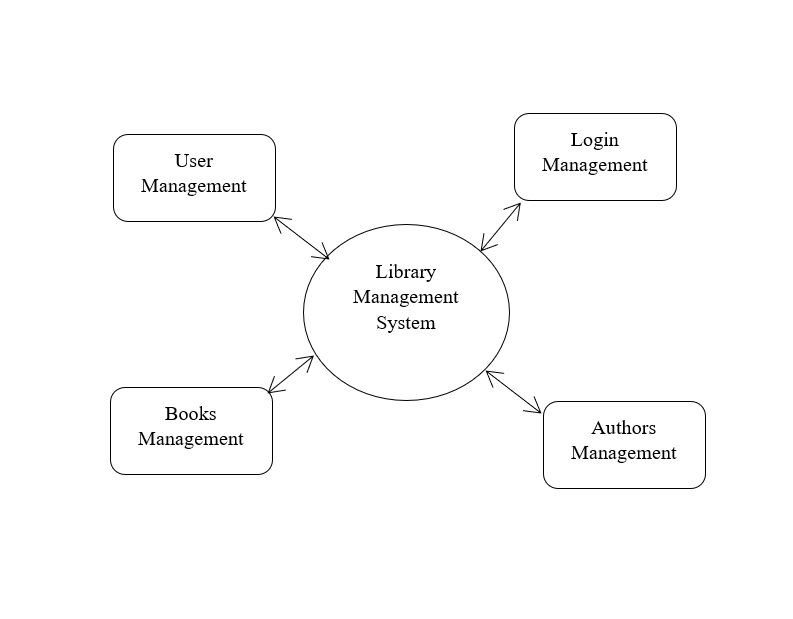
\includegraphics[scale=0.8]{./dfd-0} 
	\textbf{\caption{First Level Data Flow Diagram}}
	\label{fig:dfd1} 
\end{figure}

\newpage
\subsection{Second Level DFD}
\begin{figure}[htb]
	\centering
	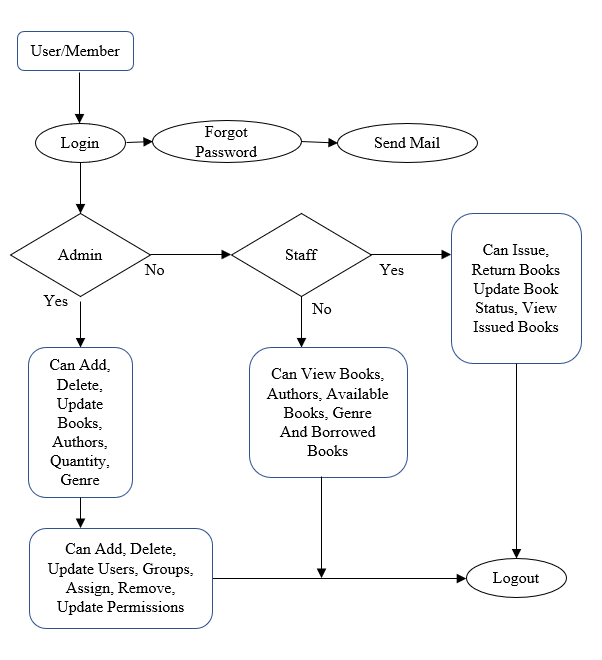
\includegraphics[scale=0.8]{./dfd-1} 
	\textbf{\caption{Second Level Data Flow Diagram}}
	\label{fig:dfd2} 
\end{figure}

\newpage
\section{Entity Relationship Diagram}

An entity relationship diagram (ERD), also known as an entity relationship model, is a graphical representation that depicts relationships among people, objects, places, concepts or events within an information technology (IT) system

Below Diagram Shows the relation between different entities in Library Management System.
\begin{figure}[htb]
	\centering
	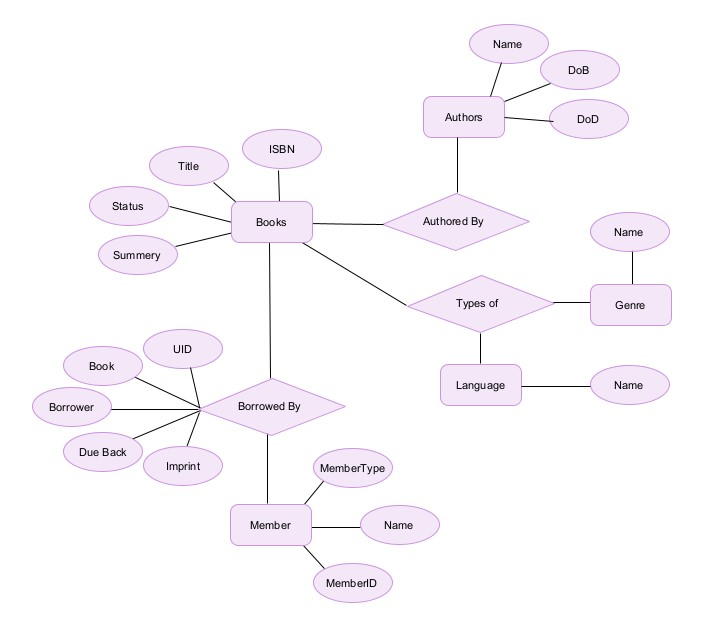
\includegraphics[scale=0.8]{./entity-relationship} 
	\textbf{\caption{Entity Relationship Design}}
	\label{fig:erd} 
\end{figure}

\newpage

\section{Sequence Diagram}

A sequence diagram is a Unified Modeling Language (UML) diagram that illustrates the sequence of messages between objects in an interaction. A sequence diagram consists of a group of objects that are represented by lifelines, and the messages that they exchange over time during the interaction.
A sequence diagram shows the sequence of messages passed between objects. Sequence diagrams can also show the control structures between objects. For example, lifelines in a sequence diagram for a library scenario can represent a user, a librarian, library computer, an books database.
The sequence diagram shows the interaction between them.

\begin{figure}[htb]
\centering
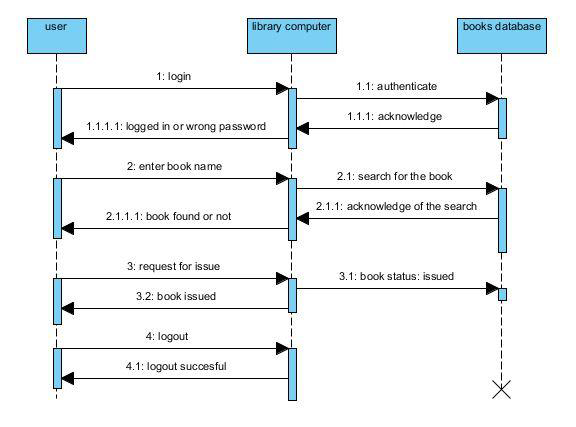
\includegraphics[scale=0.8]{./sequence-diagram} 
\textbf{\caption{Sequence Design}}
\label{fig:sequence} 
\end{figure}

\newpage
\section{Database Design}

Database design is a collection of steps that help create, implement, and maintain a business’s data management systems. The primary purpose of designing a database is to produce physical and logical models of designs for the proposed database system.


A good database design process is governed by specific rules. The first rule is to avoid data redundancy. It wastes space and increases the probability of faults and discrepancies within the database. The second rule is that the accuracy and comprehensiveness of information are imperative. 

A database designed for Library Management System show below has five table which contains information schema to store information of different entities of project.

\begin{figure}[htb]
	\centering
	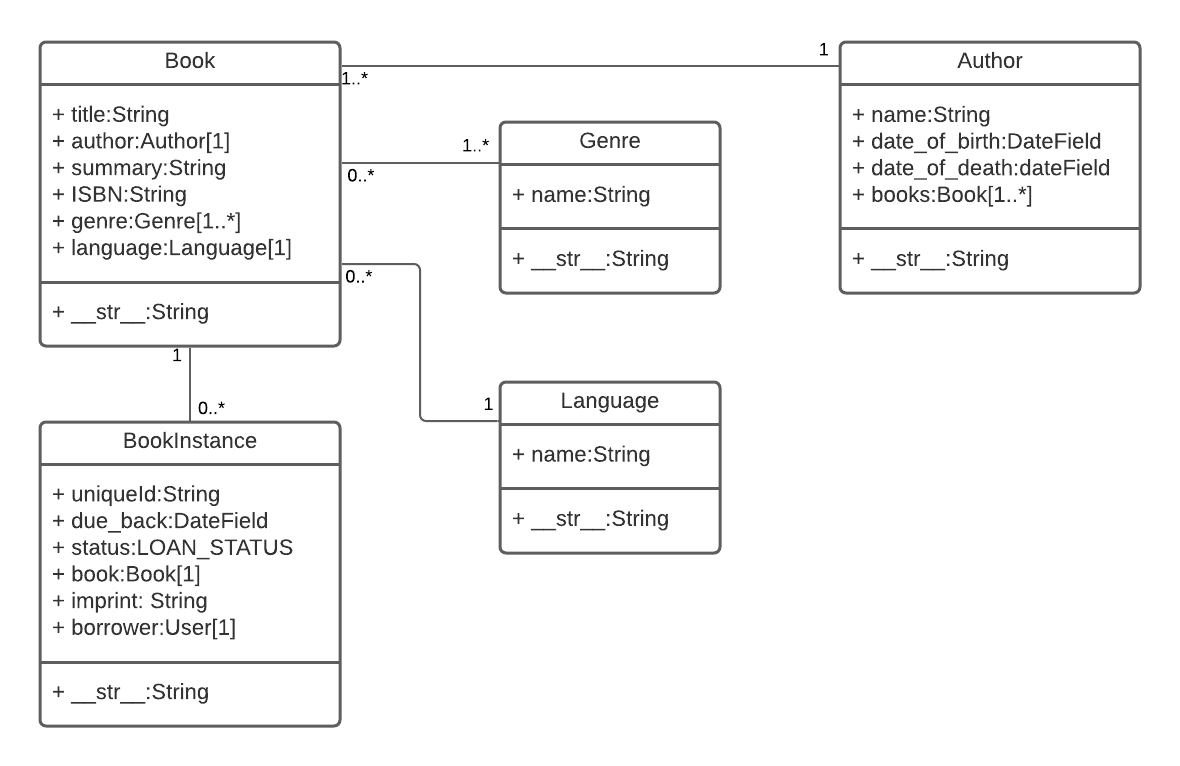
\includegraphics[scale=0.8]{./models} 
	\textbf{\caption{Database Table Design}}
	\label{fig:dbtable} 
\end{figure}

\newpage
\chapter{Implementation}
Actual Implementation starts after when have properly designed architecture and have supporting development model for implementation. Development model is used to choose the way you want to delivery your software success. There are various models that you can choose from such as waterfall model, agile model, spiral methodologies.

Now Lets talk about such development models and approaches used by them and benefits of using them. 

\subsubsection{Waterfall Model}
The Waterfall Model was the first Process Model to be introduced. It is also referred to as a linear-sequential life cycle model. It is very simple to understand and use. In a waterfall model, each phase must be completed before the next phase can begin and there is no overlapping in the phases.

The Waterfall model is the earliest SDLC approach that was used for software development.
The waterfall Model illustrates the software development process in a linear sequential flow. This means that any phase in the development process begins only if the previous phase is complete. In this waterfall model, the phases do not overlap.

Waterfall approach was first SDLC Model to be used widely in Software Engineering to ensure success of the project. In "The Waterfall" approach, the whole process of software development is divided into separate phases. In this Waterfall model, typically, the outcome of one phase acts as the input for the next phase sequentially. The following illustration is a representation of the different phases of the Waterfall Model.

\begin{figure}[htb]
	\centering
	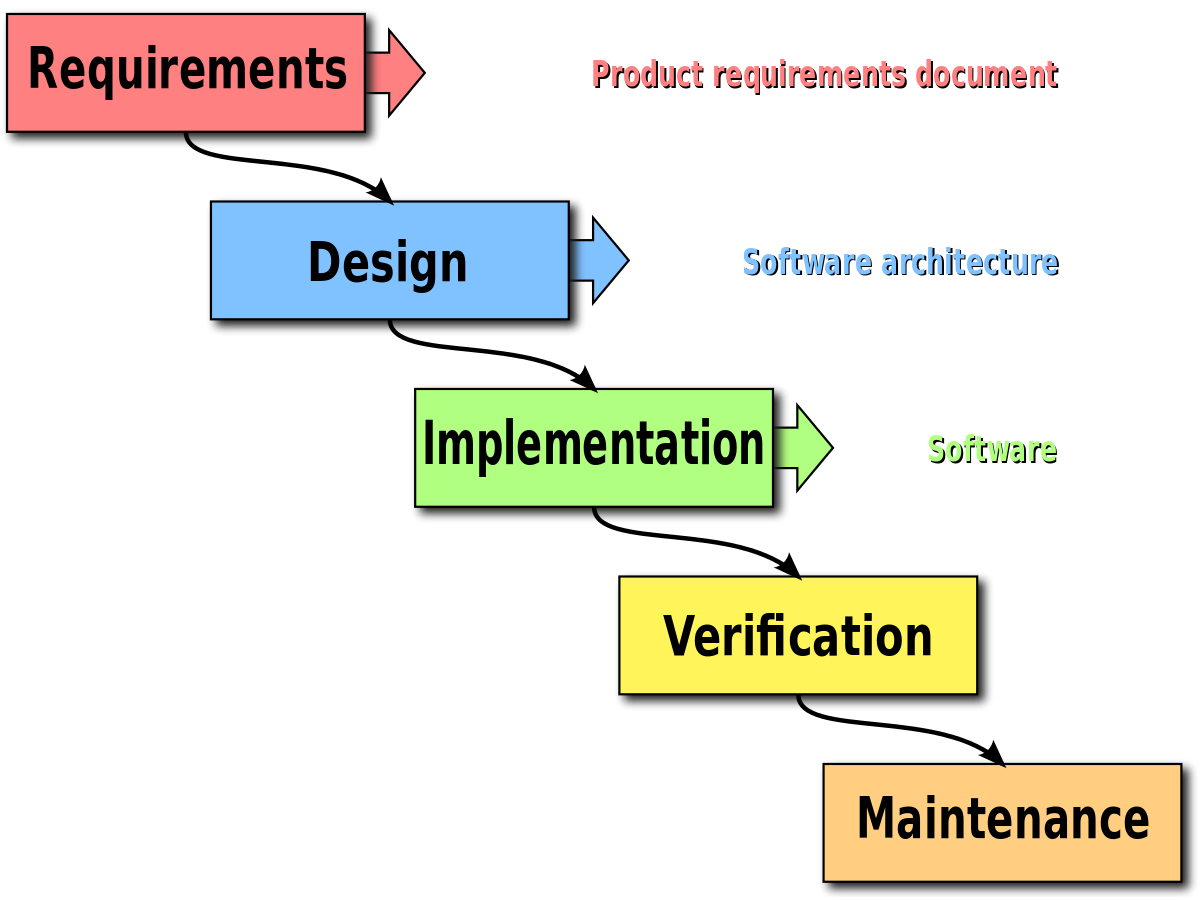
\includegraphics[scale=0.2]{./waterfall} 
	\textbf{\caption{Waterfall Model}}
	\label{fig:waterfall} 
\end{figure}

\hspace{1cm}

\newpage
\subsubsection{Agile Model}
In earlier days Iterative Waterfall model was very popular to complete a project. But nowadays developers face various problems while using it to develop software. The main difficulties included handling change requests from customers during project development and the high cost and time required to incorporate these changes. To overcome these drawbacks of Waterfall model, in the mid-1990s the Agile Software Development model was proposed. 

The Agile model was primarily designed to help a project to adapt to change requests quickly. So, the main aim of the Agile model is to facilitate quick project completion. To accomplish this task agility is required. Agility is achieved by fitting the process to the project, removing activities that may not be essential for a specific project. Also, anything that is wastage of time and effort is avoided. 

Actually Agile model refers to a group of development processes. These processes share some basic characteristics but do have certain subtle differences among themselves. A few Agile SDLC models are given below:

\begin{itemize}
	\item Crystal
	\item Feature-driven development
	\item Scrum
	\item Extreme programming (XP)
	\item Lean development
\end{itemize}


Below figure shows the clear differences between Waterfall model and Agile Model of the Development.

\begin{figure}[htb]
	\centering
	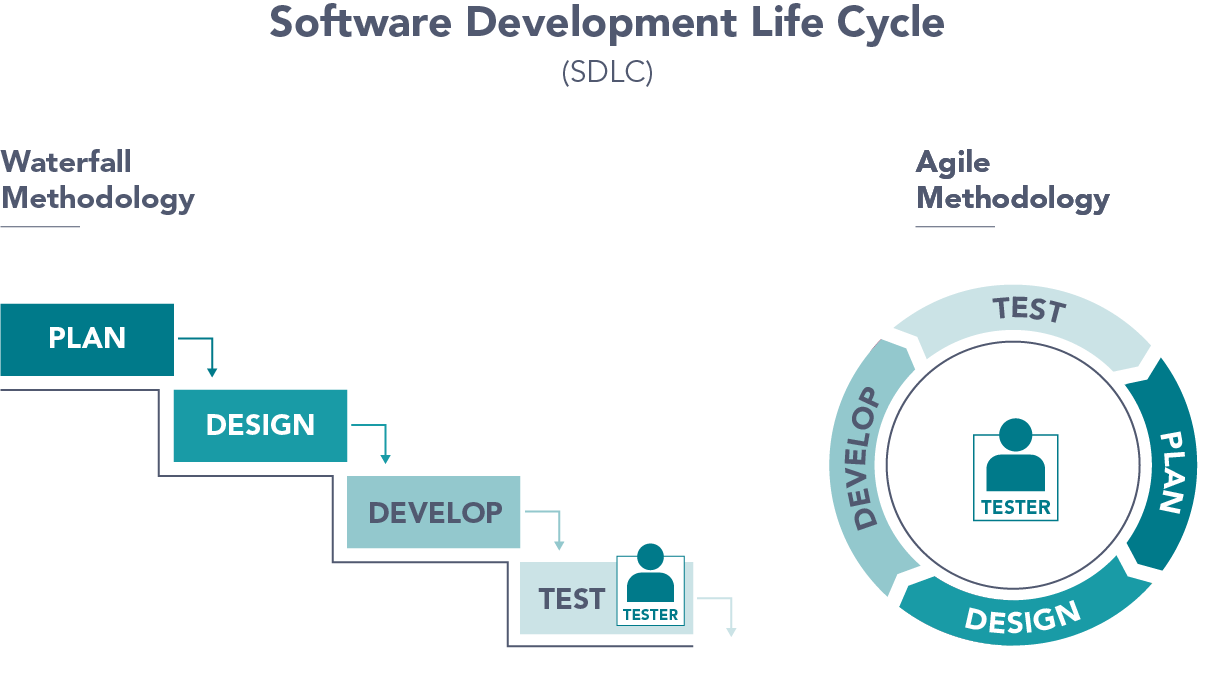
\includegraphics[scale=0.3]{./methodologies} 
	\textbf{\caption{Waterfall Model}}
	\label{fig:agile} 
\end{figure}


As we were able to see the clear picture of usage of methodologies using waterfall and agile. We have used the approach of Agile Development model to start the development of our project


\newpage
\section{User Interface}

The user interface (UI) is the point at which human users interact with a computer, website or application. The goal of effective UI is to make the user's experience easy and intuitive, requiring minimum effort on the user's part to receive maximum desired outcome.

Below User Interface is used to show how the users of the library will interarct with System
\begin{itemize}
	\item The Library record shows the number of Available to Books, Books of the Authors etc.
	\item List of Books shows the paginated list of Books available in Library.
	\item List of Authors shows the paginated list of Authors available in Library.
	\item Displays the Issued books to members of the library
	\item Books borrowed by Staff shows books taken by members other than students
\end{itemize}
\newpage
\begin{figure}[htb]
	\centering
	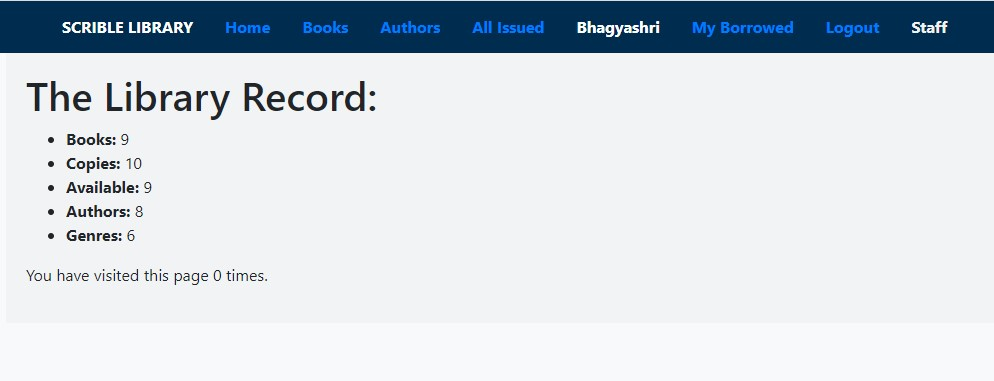
\includegraphics[scale=0.6]{./home} 
	\caption{The Library Record}
	\label{fig:librec} 
\end{figure}

\newpage
\begin{figure}[htb]
	\centering
	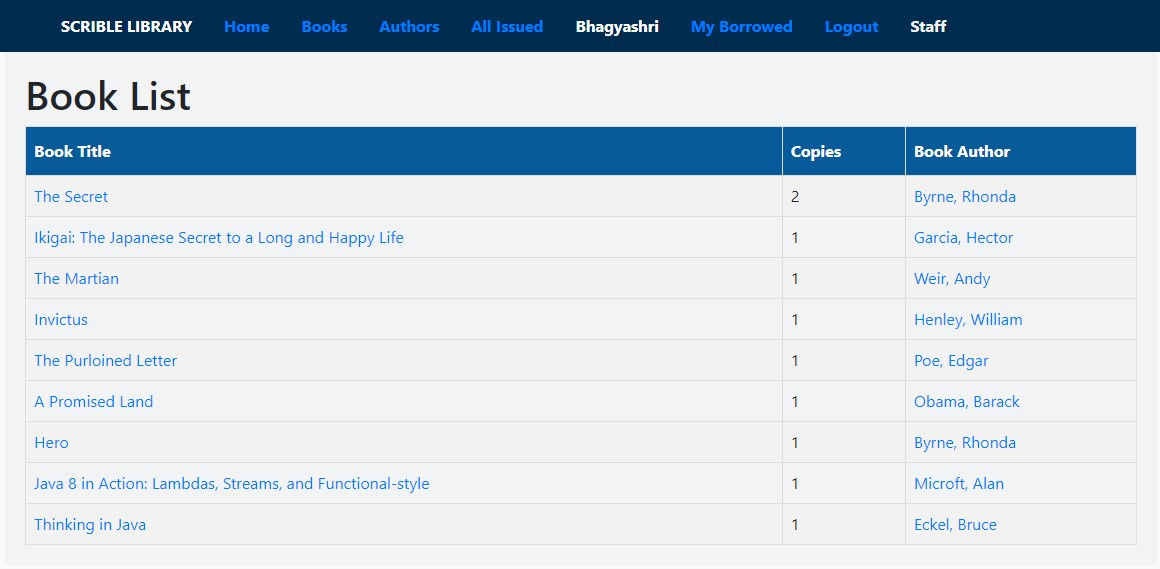
\includegraphics[scale=0.5]{./books} 
	\caption{Books List}
	\label{fig:books} 
\end{figure}
\newpage
\begin{figure}[htb]
	\centering
	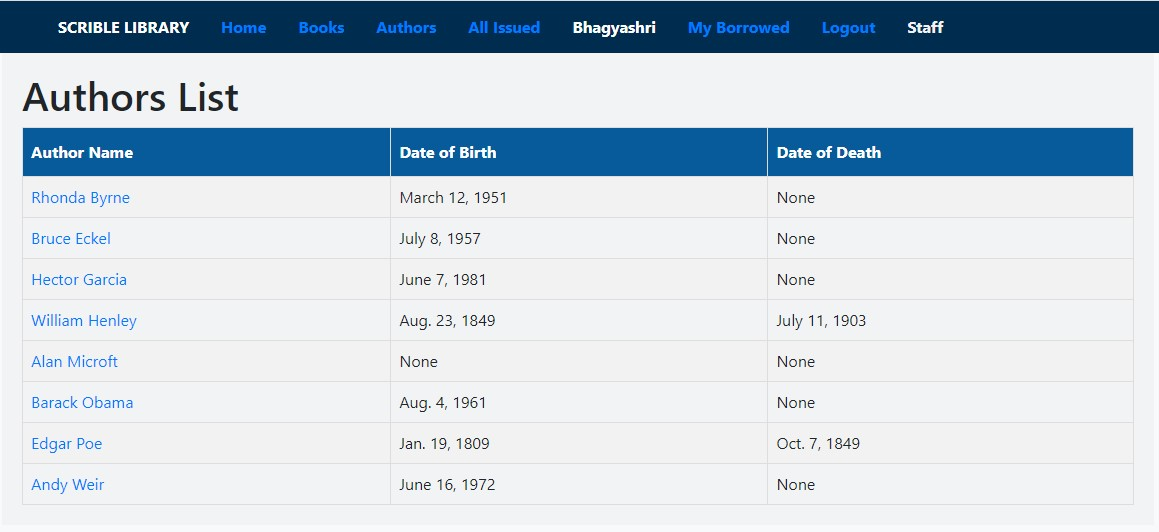
\includegraphics[scale=0.5]{./authors} 
	\caption{Authors List}
	\label{fig:listauthor} 
\end{figure}
\newpage
\begin{figure}[htb]
	\centering
	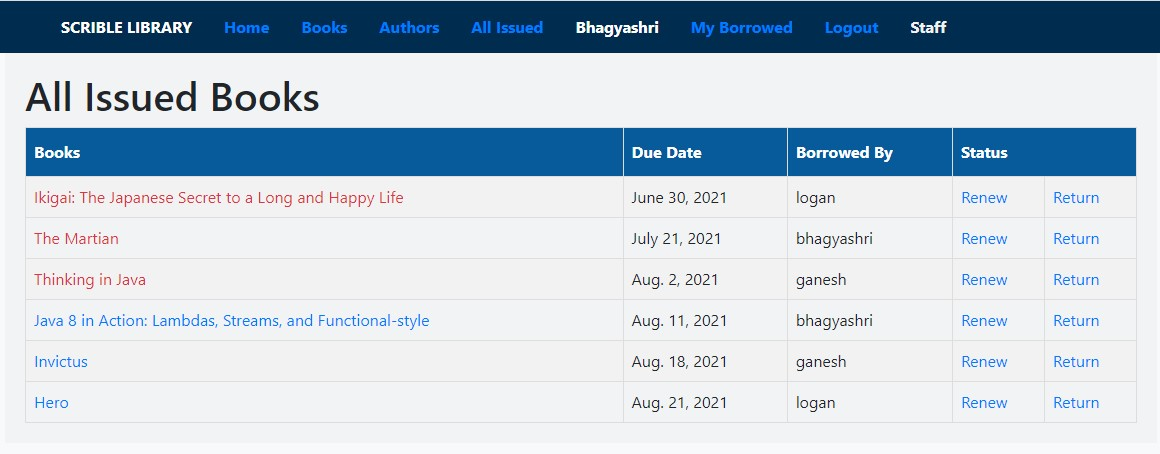
\includegraphics[scale=0.5]{./issued} 
	\caption{All Issued Books}
	\label{fig:issued} 
\end{figure}
\newpage
\begin{figure}[htb]
	\centering
	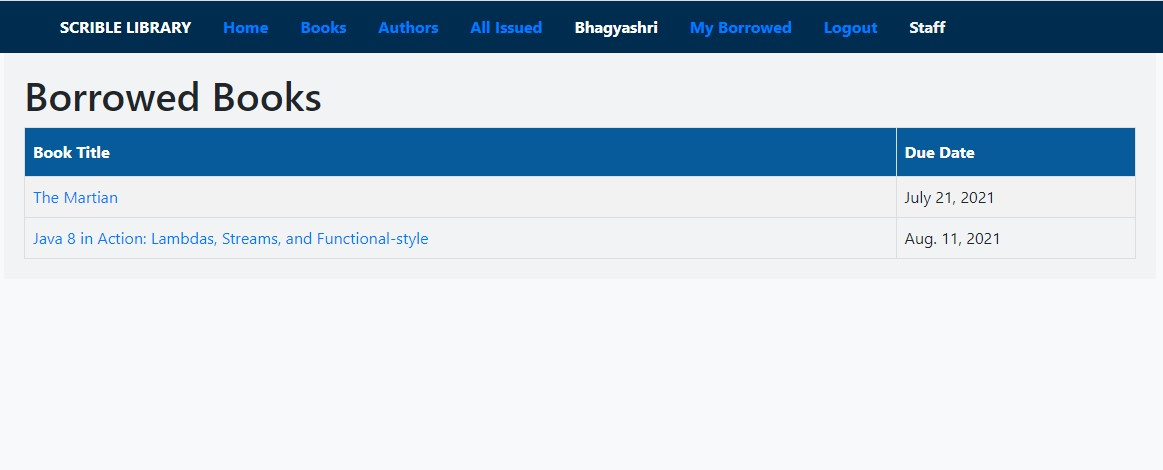
\includegraphics[scale=0.5]{./borrowed} 
	\caption{Books Borrowed By Staff}
	\label{fig:students} 
\end{figure}

\newpage
\begin{figure}[htb]
	\centering
	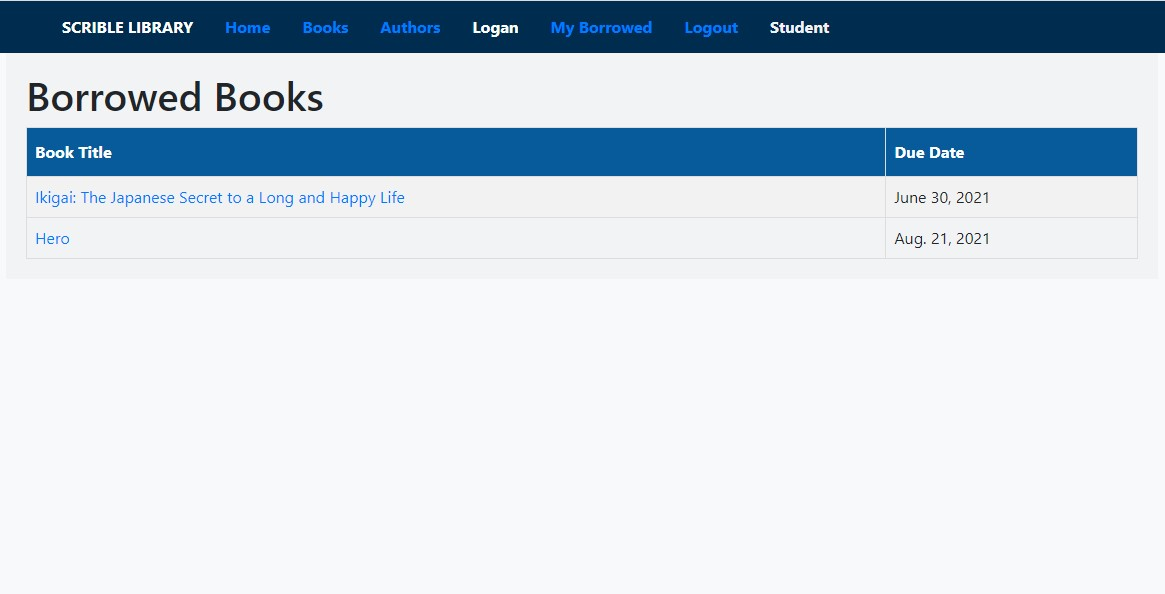
\includegraphics[scale=0.5]{./students} 
	\caption{Books Borrowed By Students}
	\label{fig:borroed} 
\end{figure}

\newpage
\section{Admin Interface}

The admin interface, often referred to as the “back end,” is a Symphony project's primary control panel. Once logged in, authors can use the admin interface to set up and configure a project, manage its structure and content, install extensions, and perform other tasks.

\par Django provides a default admin interface which can be used to perform create, read, update and delete operations on the model directly. It reads set of data that explain and gives information about data from the model, to provide an instant interface where the user can adjust contents of the application 

By using admin interface in our library we can have complete control over the application.
\begin{itemize}
	\item Admin Interface shows the homescreen of the Library Admin at first glance.
	\item Book Catalog shows the number of Book Names, Authors, etc.
	\item Add New Book to Library shows how admin adds the books in the library
	\item Similarly Add New Author to Library show way to add author in library
	\item How to delete the members from library
	\item Adding languages of the books to library.
	\item Finally how to change the password of Admin.
\end{itemize}

\newpage
\begin{figure}[htb]
	\centering
	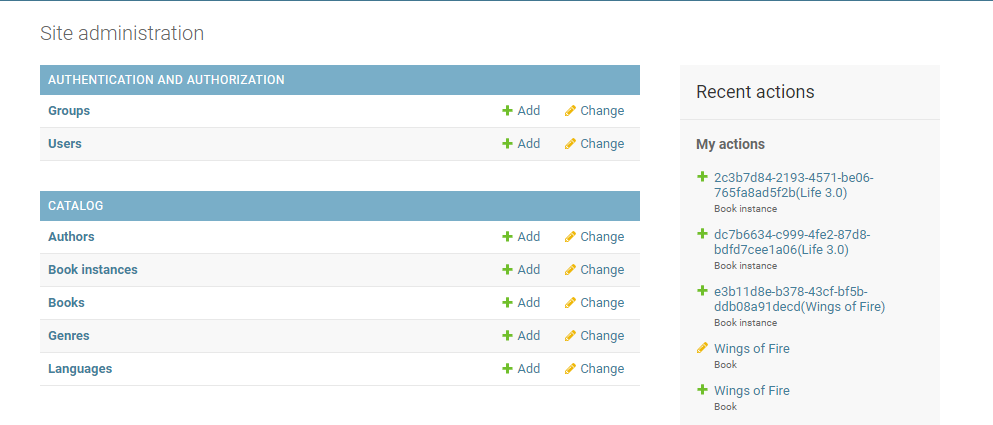
\includegraphics[scale=0.6]{./admin-interface} 
	\caption{Admin Interface}
	\label{fig:admin} 
\end{figure}

\newpage
\begin{figure}[htb]
	\centering
	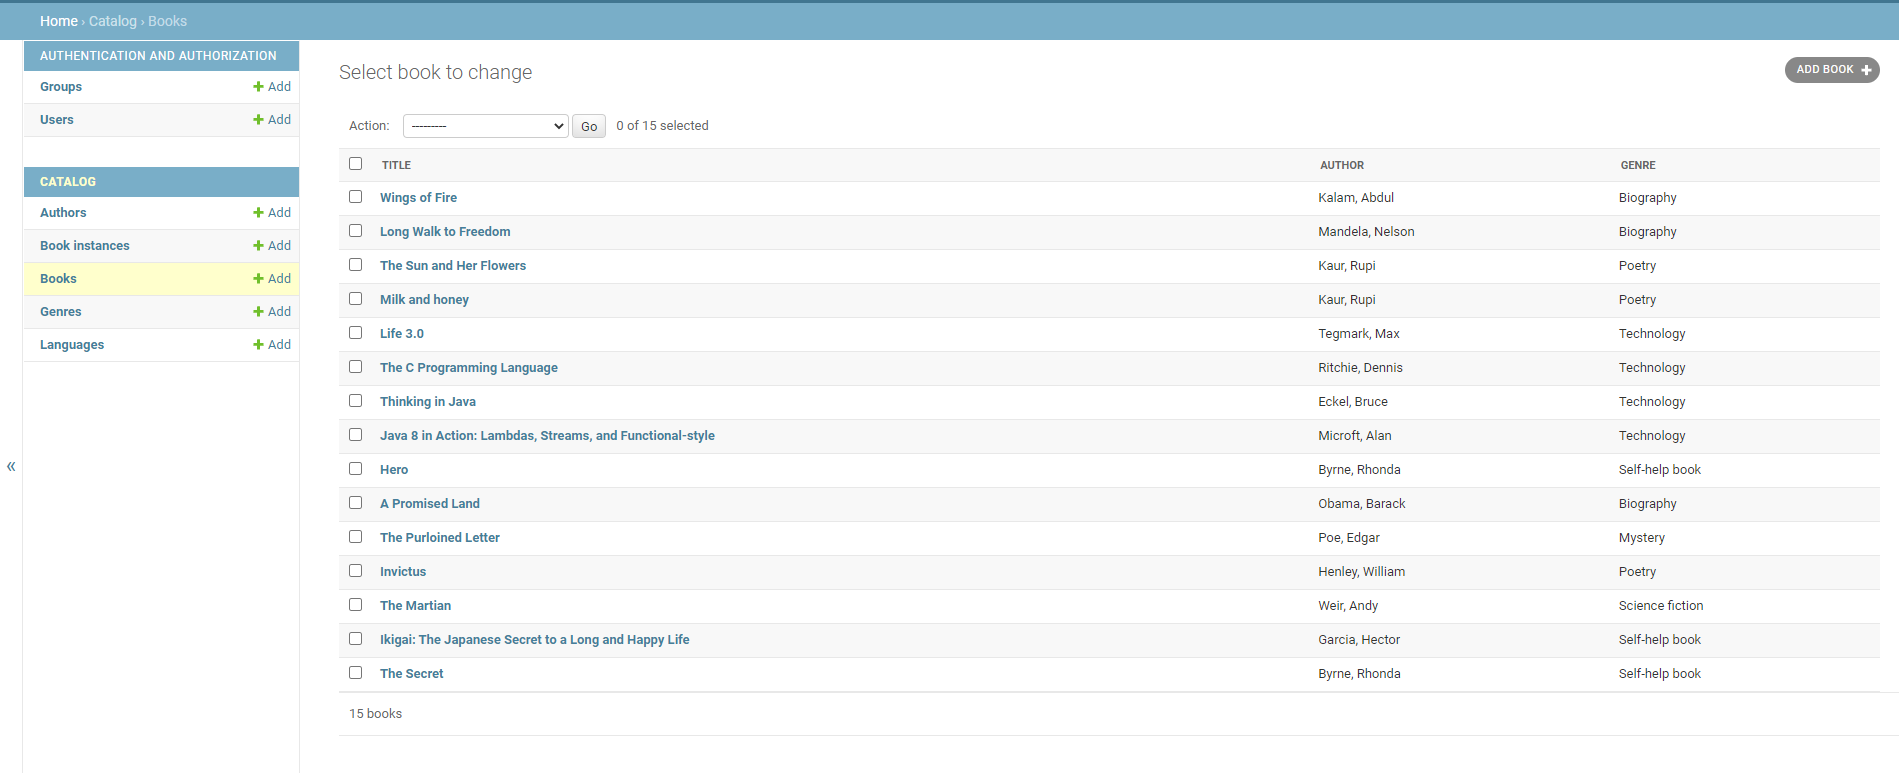
\includegraphics[scale=0.3]{./book-catalog} 
	\caption{Book Catalog}
	\label{fig:catalog} 
\end{figure}

\newpage
\begin{figure}[htb]
	\centering
	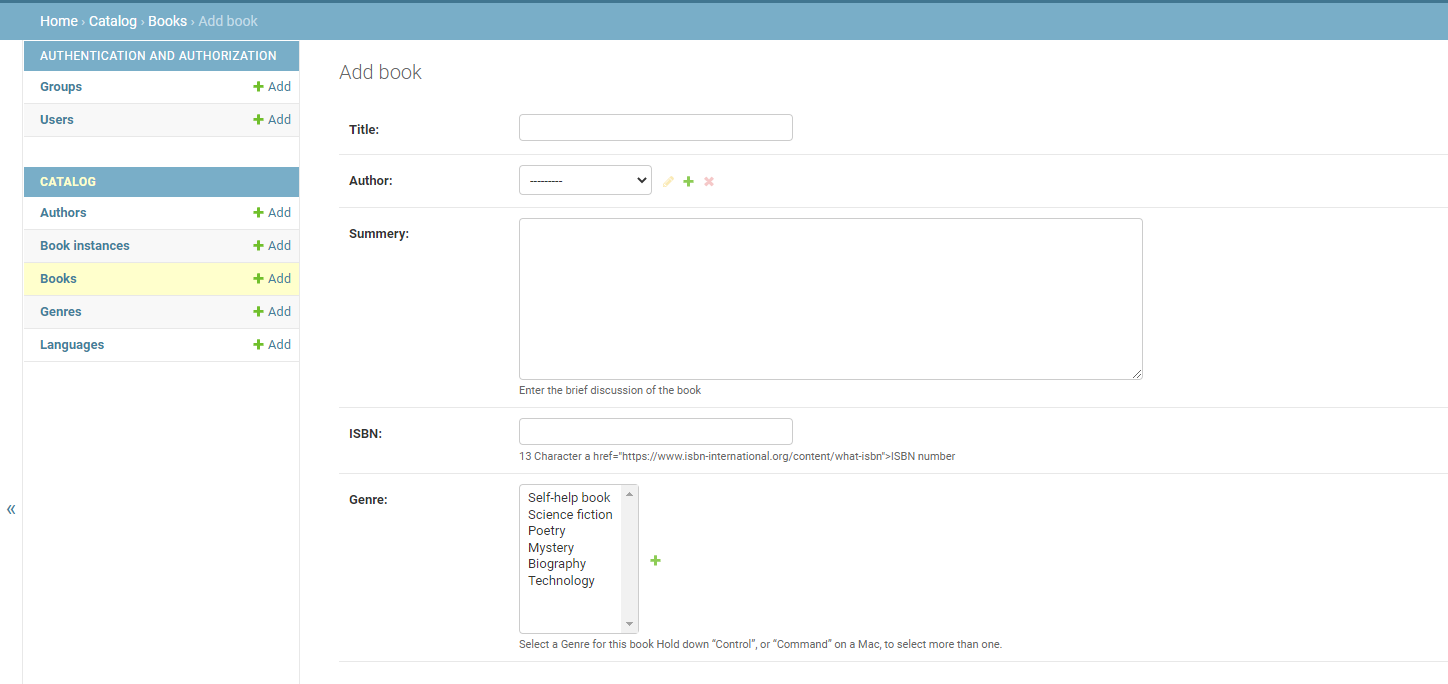
\includegraphics[scale=0.4]{./add-book} 
	\caption{Add New Book to Library}
	\label{fig:bookadd} 
\end{figure}

\newpage
\begin{figure}[htb]
	\centering
	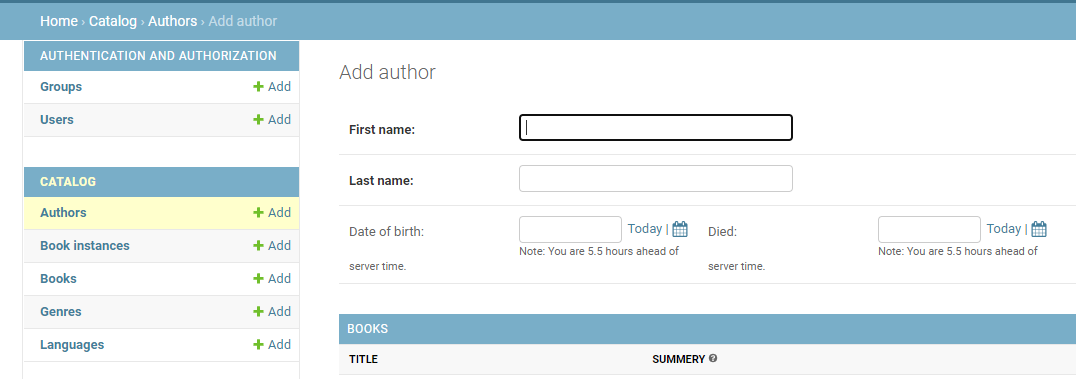
\includegraphics[scale=0.5]{./author-add} 
	\caption{Add New Author to Library}
	\label{fig:author-add} 
\end{figure}

\newpage
\begin{figure}[htb]
	\centering
	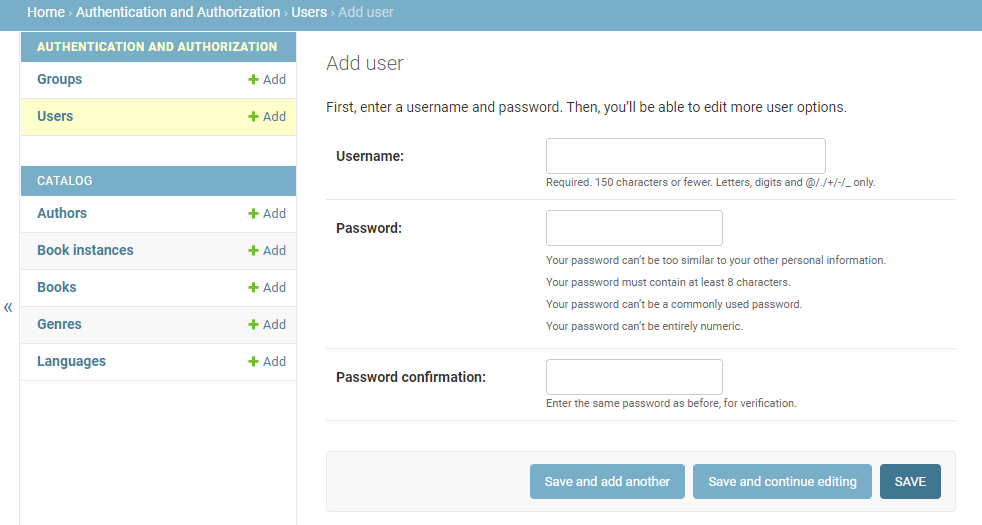
\includegraphics[scale=0.5]{./add-member} 
	\caption{Add New Member to Library}
	\label{fig:member-add} 
\end{figure}

\newpage
\begin{figure}[htb]
	\centering
	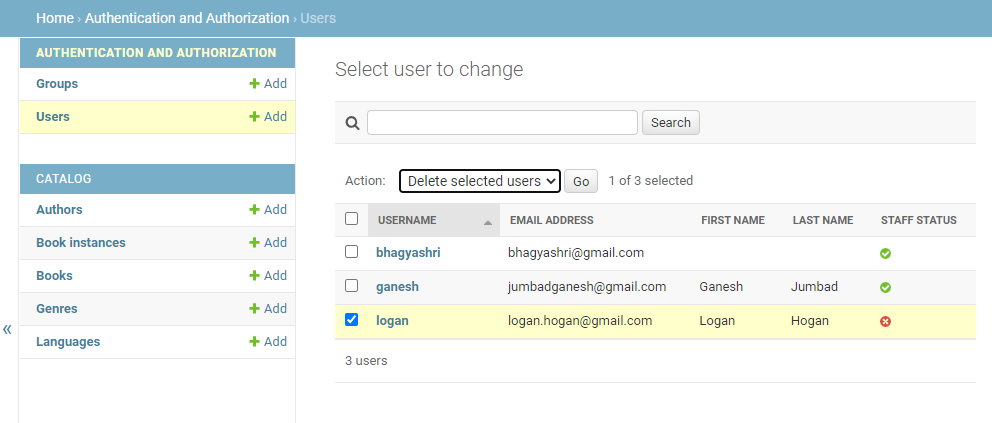
\includegraphics[scale=0.5]{./delete-member} 
	\caption{Delete Existing Member from Library}
	\label{fig:member-delete} 
\end{figure}

\newpage
\begin{figure}[htb]
	\centering
	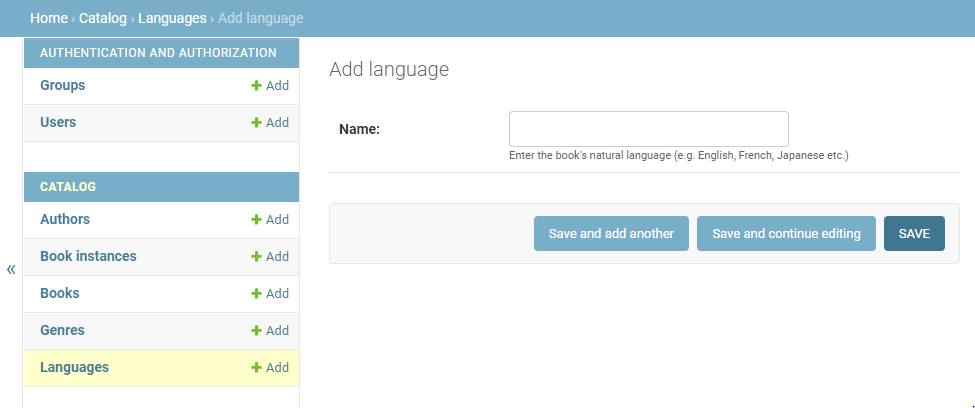
\includegraphics[scale=0.5]{./languages} 
	\caption{Add New Language for Books to Library}
	\label{fig:language-add} 
\end{figure}

\newpage
\begin{figure}[htb]
	\centering
	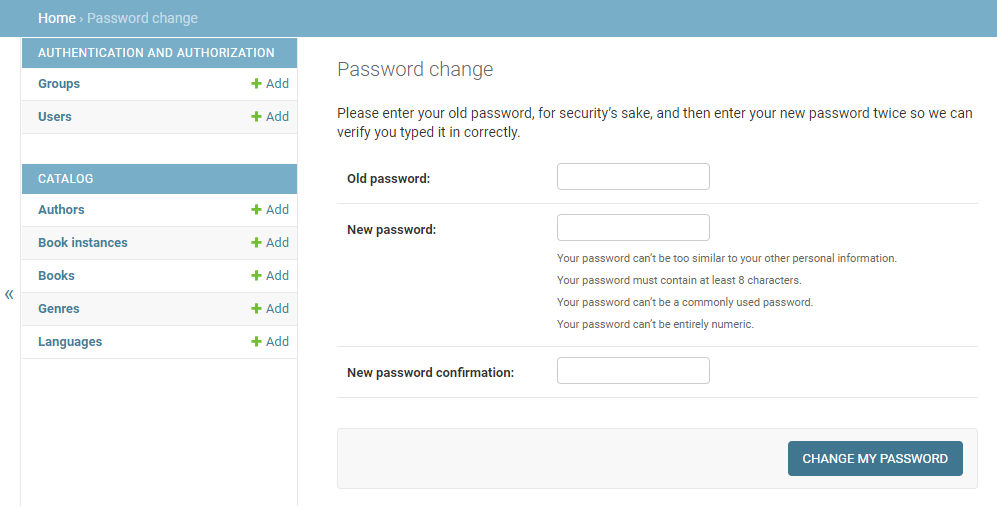
\includegraphics[scale=0.5]{./password-change} 
	\caption{Change Admin password}
	\label{fig:password-change} 
\end{figure}

\newpage
\section{Technologies Used}

In this Section we will do Analysis of Technologies to use for implementing the project.
\subsection{Front End}
\subsubsection{HTML}
Hypertext Markup Language (HTML) is the standard markup language for documents designed to
be displayed in a web browser. It can be assisted by technologies such as Cascading Style Sheets
(CSS) and scripting languages such as JavaScript.
Web browsers receive HTML documents from a
web server or from local storage and render the documents into multimedia web pages. HTML
describes the structure of a web page semantically and originally included cues for the appearance
of the document.
HTML elements are the building blocks of HTML pages.\par With HTML constructs, images and other
objects such as interactive forms may be embedded into the rendered page. HTML provides a
means to create structured documents by denoting structural semantics for text such as headings,
paragraphs, lists, links, quotes and other items. HTML elements are delineated by tags, written
using angle brackets. Tags such as img and input directly introduce content into the page.
Other tags such as p surround and provide information about document text and may include
other tags as sub-elements. Browsers do not display the HTML tags, but use them to interpret the
content of the page.
HTML can embed programs written in a scripting language such as JavaScript, which affects the
behavior and content of web pages. Inclusion of CSS defines the look and layout of content. The
World Wide Web Consortium (W3C), former maintainer of the HTML and current maintainer of the
CSS standards, has encouraged the use of CSS over explicit presentational HTML since 1997.

\subsubsection{JavaScript}
JavaScript s a high-level, interpreted scripting language that conforms to the ECMAScript
specification. JavaScript has curly-bracket syntax, dynamic typing, prototype-based objectorientation,
and first-class functions.Alongside HTML and CSS, JavaScript is one of the core
technologies of the World Wide Web. JavaScript enables interactive web pages and is an essential
part of web applications.\par The vast majority of websites use it, and major web browsers have a
dedicated JavaScript engine to execute it. As a multi-paradigm language, JavaScript supports eventdriven,
functional, and imperative (including object-oriented and prototype-based) programming
styles. It has APIs for working with text, arrays, dates, regular expressions, and the DOM, but the
language itself does not include any I/O, such as networking, storage, or graphics facilities. It relies
upon the host environment in which it is embedded to provide these features.
\par Initially only implemented client-side in web browsers, JavaScript engines are now embedded in
many other types of host software, including server-side in web servers and databases, and in nonweb
programs such as word processors and PDF software, and in runtime environments that make
JavaScript available for writing mobile and desktop applications, including desktop widgets.
The terms Vanilla JavaScript and Vanilla JS refer to JavaScript not extended by any frameworks or
additional libraries. Scripts written in Vanilla JS are plain JavaScript code.Google's Chrome
extensions, Opera's extensions, Apple's Safari 5 extensions, Apple's Dashboard Widgets, Microsoft's
Gadgets, Yahoo! Widgets, Google Desktop Gadgets, and Serence Klipfolio are implemented using
JavaScript.

\subsubsection{CSS}
Cascading Style Sheets (CSS) is a style sheet language used for describing the presentation of a
document written in a markup language like HTML.CSS is a cornerstone technology of the World
Wide Web, alongside HTML and JavaScript.CSS is designed to enable the separation of
presentation and content, including layout, colors, and fonts.This separation can improve content
accessibility, provide more flexibility and control in the specification of presentation characteristics,
enable multiple web pages to share formatting by specifying the relevant CSS in a separate .css file,
and reduce complexity and repetition in the structural content.
\par One of the goals of CSS is to allow users greater control over presentation. Someone who finds red
italic headings difficult to read may apply a different style sheet. Depending on the browser and the
web site, a user may choose from various style sheets provided by the designers, or may remove all
added styles and view the site using the browser's default styling, or may override just the red italic
heading style without altering other attributes.


\subsection{Backend}
\subsubsection{Python}
Python is an interpreted, high-level, general-purpose programming language. Created by \textbf{Guido van
	Rossum} and first released in 1991, Python's design philosophy emphasizes code readability with its
notable use of significant whitespace. Its language constructs and object-oriented approach aim to
help programmers write clear, logical code for small and large-scale projects.Python is dynamically
typed and garbage-collected. It supports multiple programming paradigms, including procedural,
object-oriented, and functional programming. Python is often described as a "batteries included"
language due to its comprehensive standard library.
\par Python was conceived in the late 1980s as a successor to the ABC language. Python 2.0, released
2000, introduced features like list comprehensions and a garbage collection system capable of
collecting reference cycles. Python 3.0, released 2008, was a major revision of the language that is
not completely backward-compatible, and much Python 2 code does not run unmodified on Python
3. Due to concern about the amount of code written for Python 2, support for Python 2.7 (the last
release in the 2.x series) was extended to 2020. Language developer Guido van Rossum shouldered
sole responsibility for the project until July 2018 but now shares his leadership as a member of a
five-person steering council.
\par Python interpreters are available for many operating systems. A global community of programmers
develops and maintains CPython, an open source[32] reference implementation. A non-profit
organization, the Python Software Foundation, manages and directs resources for Python and
CPython development.

\subsubsection{Django}
Django is a high-level Python web framework that enables rapid development of secure and maintainable websites. Built by experienced developers, Django takes care of much of the hassle of web development, so you can focus on writing your app without needing to reinvent the wheel. It is free and open source, has a thriving and active community, great documentation, and many options for free and paid-for support. \newline Django helps you write software that is:
\begin{itemize}
	\item Complete - Django follows the "Batteries included" philosophy and provides almost everything developers might want to do "out of the box". Because everything you need is part of the one "product", it all works seamlessly together, follows consistent design principles, and has extensive and up-to-date documentation.
	\item Versatile - Django can be (and has been) used to build almost any type of website — from content management systems and wikis, through to social networks and news sites. It can work with any client-side framework, and can deliver content in almost any format (including HTML, RSS feeds, JSON, XML, etc). The site you are currently reading is built with Django!
	\item Secure - Django helps developers avoid many common security mistakes by providing a framework that has been engineered to "do the right things" to protect the website automatically. For example, Django provides a secure way to manage user accounts and passwords, avoiding common mistakes like putting session information in cookies where it is vulnerable (instead cookies just contain a key, and the actual data is stored in the database) or directly storing passwords rather than a password hash.
	
	\item Scalable - Django uses a component-based “shared-nothing” architecture (each part of the architecture is independent of the others, and can hence be replaced or changed if needed). Having a clear separation between the different parts means that it can scale for increased traffic by adding hardware at any level: caching servers, database servers, or application servers. Some of the busiest sites have successfully scaled Django to meet their demands (e.g. Instagram and Disqus, to name just two).
	\item Maintainable - Django code is written using design principles and patterns that encourage the creation of maintainable and reusable code. In particular, it makes use of the Don't Repeat Yourself (DRY) principle so there is no unnecessary duplication, reducing the amount of code. Django also promotes the grouping of related functionality into reusable "applications" and, at a lower level, groups related code into modules (along the lines of the Model View Controller (MVC) pattern).
	\item Portable - Django is written in Python, which runs on many platforms. That means that you are not tied to any particular server platform, and can run your applications on many flavours of Linux, Windows, and Mac OS X. Furthermore, Django is well-supported by many web hosting providers, who often provide specific infrastructure and documentation for hosting Django sites.
\end{itemize}

\subsubsection{SQLite}
SQLite is a relational database management system (RDBMS) contained in a C library. In contrast to many other database management systems, SQLite is not a client–server database engine. Rather, it is embedded into the end program.

\par SQLite generally follows PostgreSQL syntax. SQLite uses a dynamically and weakly typed SQL syntax that does not guarantee the domain integrity. This means that one can, for example, insert a string into a column defined as an integer. SQLite will attempt to convert data between formats where appropriate, the string "123" into an integer in this case, but does not guarantee such conversions and will store the data as-is if such a conversion is not possible.

\par SQLite is a popular choice as embedded database software for local/client storage in application software such as web browsers. It is arguably the most widely deployed database engine, as it is used today by several widespread browsers, operating systems, and embedded systems (such as mobile phones), among others. SQLite has bindings to many programming languages.


\par SQLite is used almost everywhere from features phones to satellites etc. There are many applications of SQLite such as in Middleware, WebBrowsers, Web Application Framework, Mobile Operating Systems such as Blackberry OS, Android OS, Symbian OS, Linux, Windows etc. Also various Applications such as Adobe Photoshop Lightroom, Apple Photos, Evernote, Skype etc. Programming Languages such as python, AppleScript, Kotlin, Java etc.

\newpage
\subsection{Development Tools Used}

Integrated Development Environment tools are necessary to develop any big application in any programming language. We have used below compatible tools to develop Library Application. 
\subsubsection{Visual Studio Code}
Visual Studio Code is an integrated development environment made by Microsoft for Windows, Linux and macOS. Features include support for debugging, syntax highlighting, intelligent code completion, snippets, code refactoring, and embedded Git. Users can change the theme, keyboard shortcuts, preferences, and install extensions that add additional functionality.

Microsoft has released most of Visual Studio Code's source code on GitHub under the permissive MIT License, while the releases by Microsoft are proprietary freeware.

In the Stack Overflow 2021 Developer Survey, Visual Studio Code was ranked the most popular developer environment tool, with 70\% of 82,000 respondents reporting that they use it.

Visual Studio Code was first announced on April 29, 2015, by Microsoft at the 2015 Build conference. A preview build was released shortly thereafter. On November 18, 2015, the source of Visual Studio Code was released under the MIT License, and made available on GitHub. Extension support was also announced. On April 14, 2016, Visual Studio Code graduated from the public preview stage and was released to the Web.
\subsubsection{Visual Paradigm}

Visual Paradigm is a Design and Management Tool for Business IT System Development. In this lecture, we aim to give you a brief explanation on the 5 steps of software development, namely, requirement capturing, system design, coding as well as testing and how Visual paradigm can help to manage users’ requirements and tasks effectively.

There are 3 major user interface components in Visual Paradigm, namely, Menu bar \& toolbar, diagramming area and tree and property panes. In this lecture, we would like to brief you on each of the component and give demonstrations on different panes like Diagram Overview Pane, Stencil Pane and Documentation pane, so that you can have more ideas on how to operate Visual Paradigm and can make full use of it.

Visual Paradigm is a UML CASE Tool supporting UML 2, SysML and Business Process Modeling Notation from the Object Management Group. In addition to the modeling support, it provides report generation and code engineering capabilities including code generation.


\subsubsection{LaTex}

LaTeX is a high-quality typesetting system; it includes features designed for the production of technical and scientific documentation. LaTeX is the de facto standard for the communication and publication of scientific documents. LaTeX is available as free software.

The LaTex tool and its library are available for free i.e., there are no license fees, etc. But you are, of course, invited to support the maintenance and development efforts through a donation to the TeX Users Group (choose LaTeX Project contribution) if you are satisfied with LaTeX.


\textbf{Key Features of LaTex Documentation Tools:}
\begin{itemize}
	\item Typesetting journal articles, technical reports, books, and slide presentations.
	\item Control over large documents containing sectioning, cross-references, tables and figures.
	\item Typesetting of complex mathematical formulas.
	\item Advanced typesetting of mathematics with AMS-LaTeX.
	\item Automatic generation of bibliographies and indexes.
	\item Multi-lingual typesetting.
	\item Inclusion of artwork, and process or spot colour.
	\item Using PostScript or Metafont fonts.
\end{itemize}

\newpage
\subsubsection{Chrome Browser}

Google Chrome is a cross-platform web browser developed by Google. It was first released in 2008 for Microsoft Windows built with free software components from Apple WebKit and Mozilla Firefox. It was later ported to Linux, macOS, iOS, and Android where it is the default browser built into the OS. The browser is also the main component of Chrome OS, where it serves as the platform for web applications.

Most of Chrome's source code comes from Google's free and open-source software project Chromium, but Chrome is licensed as proprietary freeware. WebKit was the original rendering engine, but Google eventually forked it to create the Blink engine; all Chrome variants except iOS now use Blink.

As of July 2021, StatCounter estimates that Chrome has a 65\% worldwide browser market share (after peaking at 72.38\% in November 2018) on personal computers (PC), is most used on tablets (has surpassed Safari), and is also dominant on smartphones, and at 63.59\% across all platforms combined. Because of this success, Google has expanded the "Chrome" brand name to other products: Chrome OS, Chromecast, Chromebook, Chromebit, Chromebox, and Chromebase.
Some Prominent and mostly used features:
\begin{itemize}
	\item Bookmarks and settings synchronization
	\item Web standards support
	\item Malware blocking and ad blocking
	\item Incognito Mode
	\item Desktop shortcuts and apps
	\item Automatic web page translation
\end{itemize}

\newpage
\section{Coding}

\subsection{Genre Table Code}
\begin{lstlisting}
	class Genre(models.Model):
		"""Model represeting book genre"""
	
		name = models.CharField(max_length=200, help_text="Enter the genre of the Book (e.g 	Science Fiction)")
	
		def __str__(self):
			"""String for reprenting the model Object"""
			return self.name

\end{lstlisting}
\newpage
\subsection{Language Table Code}
\begin{lstlisting}
	class Language(models.Model):
		"""Model representing a Language (e.g. English, French, Japanese, etc.)"""
		name = models.CharField(max_length=200, help_text="Enter the book's natural language (e.g. English, French, Japanese etc.)")
	
		def __str__(self):
		"""String for representing the Model object (in Admin site etc.)"""
		return self.name
	
\end{lstlisting}
\newpage
\subsection{Book Table Code}
\begin{lstlisting}
	
	class Book(models.Model):
		"""Model representing the book (but not a specific copy of a book)"""
	
		title = models.CharField(max_length=200)
		author = models.ForeignKey('Author', on_delete=models.SET_NULL, null=True)
		summery = models.TextField(max_length=1000, help_text="Enter the brief discussion of 	the book")
		isbn = models.CharField('ISBN', max_length=13, unique=True, help_text='13 Character a 	href="https://www.isbn-international.org/content/what-isbn">ISBN number</a>')
		genre = models.ManyToManyField(Genre, help_text="Select a Genre for this book")
	
		def __str__(self):
			return self.title
	
		def get_absolute_url(self):
			"""Returns the URL to access a detail record for this book"""
			return reverse('book_detail', args=[str(self.id)])
		def display_genre(self):
			"""Create a string for the Genre. This is required to display genre in Admin."""
			return ', '.join(genre.name for genre in self.genre.all()[:3])
	
		display_genre.short_description = 'Genre'
\end{lstlisting}
\newpage
\subsection{BookInstance Table Code}
\begin{lstlisting}
	class BookInstance(models.Model):
		"""Model representing a specific copy of a Book"""
	
		id = models.UUIDField(primary_key=True, default=uuid.uuid4, help_text='Unique ID for 	this particular book across whole library')
		book = models.ForeignKey('Book', null=True, on_delete=models.CASCADE)
		imprint = models.CharField(max_length=200)
		due_back = models.DateField(null=True, blank=True)
		borrower = models.ForeignKey(User, on_delete=models.SET_NULL, null=True, blank=True)
	
		@property
		def is_overdue(self):
			if self.due_back and date.today() > self.due_back:
			return True
			return False
	
	
		LOAN_STATUS = (
		('m', 'Maintenance'),
		('o', 'On loan'),
		('a', 'Available'),
		('r', 'Reserved'),
		)
	
		status = models.CharField(max_length=1, choices=LOAN_STATUS, blank=True, default='a', 	help_text='Book Availability')
	
		class Meta():
			ordering = ['due_back']
			permissions = (("can_mark_returned", "Set book as returned"),)
	
		def __str__(self):
			"""String for representing the model Object"""
	
			return f'{self.id}({self.book.title})'
	
\end{lstlisting}

\subsection{Author Table Code}
\begin{lstlisting}
	
	class Author(models.Model):
		""" Model representing an Author"""
		first_name = models.CharField(max_length=100)
		last_name = models.CharField(max_length=100)
		date_of_birth = models.DateField(null=True, blank=True)
		date_of_death = models.DateField('Died', null=True, blank=True)
	
	
	class Meta:
		ordering = ['last_name', 'first_name']
	
		def get_absolute_url(self):
			"""Returns the url to access the particular instance of the Author"""
		return reverse('author-details', args=[str(self.id)])
		def __str__(self):
		"""String for representing the model object"""
		return f'{self.last_name}, {self.first_name}'
	
\end{lstlisting}
\chapter{Performance Evaluation}

Performance of the system can be evaluated using various ways. Software testing is one of them.
Software testing is the dangerous element of software excellence assurance and represents
the ultimate review of condition, design and code generation. \par Testing a projector
any software system forms the backbone of good software system. Tests are
con-ducted on the software to and out errors and bugs and remove them. Test plans
are created with a view to remove errors that can plague or hamper the project in case
the errors are encountered in runtime environment. \par Testing helps in enhancing the
overall quality of the product as it helps in removal of errors, which in turn increase
its quality. Testing is a process used to help identify the correctness, completeness
and quality of developed computer software. This document is a procedural guide
for listing the testing activities that should be carried out for proposed system.

The Purpose and objective is:
\begin{itemize}
	\item Identify all the activities involved in testing.
	\item Try to break down the system by giving it a variety of values with a view and
	hidden bugs.
	\item Testing every module in project at the internal level as well as the boundary
	level.
	\item Using various testing tools and strategies like black box and white box testing.
	\item Removing errors and testing again for any unforeseen changes in the entire
	software product.
	\item Checking the life cycle of the project and devising means to extend it.
	\item Removing inter-dependencies amongst modules such that in case of an error,
	all other modules are not defected.
	\item It also explains the strategy and approach for testing the software components
	and the defect tracking system to be used.
\end{itemize}


\section{System Testing}
System testing of software or hardware is testing conducted on a complete, integrated system to
evaluate the system's compliance with its specified requirements. System testing falls within the
scope of black-box testing, and as such, should require no knowledge of the inner design of the code
or logic. \par As a rule, system testing takes, as its input, all of the "integrated" software components that have passed integration testing and also the software system itself integrated with any applicable
hardware system(s). The purpose of integration testing is to detect any inconsistencies between the
software units that are integrated together (called assemblages) or between any of
the assemblages and the hardware. \par System testing is a more limited type of testing; it seeks to detect
defects both within the "inter-assemblages" and also within the system as a whole.
System testing is performed on the entire system in the context of a Functional
Requirement Specification(s) (FRS) and/or a System Requirement Specification (SRS). System
testing tests not only the design, but also the behavior and even the believed expectations of the
customer. It is also intended to test up to and beyond the bounds defined in the software/hardware
requirements specification(s).

\newpage
\section{Black Box Testing}

Black Box Testing is a software testing method in which the functionalities of software applications are tested without having knowledge of internal code structure, implementation details and internal paths. Black Box Testing mainly focuses on input and output of software applications and it is entirely based on software requirements and specifications. It is also known as Behavioral Testing.

The above Black-Box can be any software system you want to test. For Example, an operating system like Windows, a website like Google, a database like Oracle or even your own custom application. Under Black Box Testing, you can test these applications by just focusing on the inputs and outputs without knowing their internal code implementation. 
Here are the generic steps followed to carry out any type of Black Box Testing.
\begin{itemize}
	\item Initially, the requirements and specifications of the system are examined.
	\item Tester chooses valid inputs (positive test scenario) to check whether SUT processes them correctly. Also, some invalid inputs (negative test scenario) are chosen to verify that the SUT is able to detect them.
	\item Tester determines expected outputs for all those inputs.
	\item Software tester constructs test cases with the selected inputs.
	\item The test cases are executed.
	\item Software tester compares the actual outputs with the expected outputs.
	\item Defects if any are fixed and re-tested.
	
\end{itemize}

\newpage
\subsection{Types of Black Box Testing}
There are many types of Black Box Testing but the following are the prominent ones -
\begin{itemize}
	\item \textbf{Functional testing} - This black box testing type is related to the functional requirements of a system; it is done by software testers.
	\item \textbf{Non-functional testing} - This type of black box testing is not related to testing of specific functionality, but non-functional requirements such as performance, scalability, usability.
	\item \textbf{Regression testing} - Regression Testing is done after code fixes, upgrades or any other system maintenance to check the new code has not affected the existing code.
	
\end{itemize}

\section{Testing Strategy}

A Test Strategy is a plan for defining an approach to the Software Testing Life Cycle (STLC). It guides teams to define Test Coverage and testing scope. It helps testers get a clear picture of the project at any instance. The possibility of missing any test activity is very low when there is a proper test strategy in place.


Following figure shows the generic idea and work stages for Testing any software

\begin{figure}[htb]
	\centering
	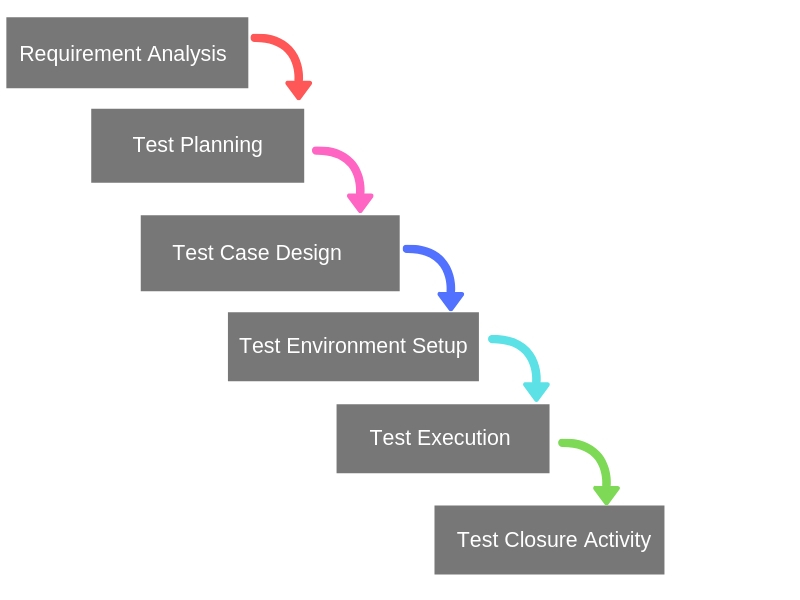
\includegraphics[scale=0.4]{./testcylce} 
	\textbf{\caption{Generic Steps for Software Testing}}
	\label{fig:test-cycle} 
\end{figure}
\newpage
\subsection{Test Strategy Document}
Test Strategy Document is a well-described document in software testing which clearly defines the exact software testing approach and testing objectives of the software application. Test document is an important document for QA teams which is derived from actual business requirements that guides the whole team about software testing approach and objectives for each activity in the software testing process.

A Test strategy document answers all the questions like what you want to get done and how you are going to accomplish it, etc. Writing an effective Strategy document is a skill that a tester develops with experience. Testing strategy plan should be communicated with the entire team so that the team will be consistent on approach and responsibilities.\newline
Following are the prominent Test Strategy used in Black box Testing
\begin{enumerate}
	\item \textbf{Equivalence Class Testing:} It is used to minimize the number of possible test cases to an optimum level while maintains reasonable test coverage.
	\item \textbf{Boundary Value Testing:} Boundary value testing is focused on the values at boundaries. This technique determines whether a certain range of values are acceptable by the system or not. It is very useful in reducing the number of test cases. It is most suitable for the systems where an input is within certain ranges.
	\item \textbf{Decision Table Testing}: A decision table puts causes and their effects in a matrix. There is a unique combination in each column.

\end{enumerate}

\newpage
\subsection{Unit Testing}
A unit test is a piece of a code (usually a method) that invokes another piece of code and checks the correctness of some assumptions afterward. If the assumptions turn out to be wrong, the unit test has failed. A unit is a method or function.

\par Unit testing is an essential instrument in the toolbox of any serious software developer. However, it can sometimes be quite difficult to write a good unit test for a particular piece of code. Having difficulty testing their own or someone else’s code, developers often think that their struggles are caused by a lack of some fundamental testing knowledge or secret unit testing techniques.
Project specific testing libraries for Python used as below:
\subsubsection{unittest — Unit testing framework}
The unittest unit testing framework was originally inspired by JUnit and has a similar flavor as major unit testing frameworks in other languages. It supports test automation, sharing of setup and shutdown code for tests, aggregation of tests into collections, and independence of the tests from the reporting framework.

\subsubsection{pytest - Another Unit testing framework}
The pytest framework makes it easy to write small tests, yet scales to support complex functional testing for applications and libraries and has following features.
\begin{itemize}
	\item Detailed info on failing assert statements (no need to remember self.assert* names)
	\item Auto-discovery of test modules and functions
	\item Modular fixtures for managing small or parametrized long-lived test resources
	\item Can run unittest (or trial), nose test suites out of the box
	\item Python 3.6+ and PyPy3
	\item Rich plugin architecture, with over 850+ external plugins and thriving community
\end{itemize}

\newpage
\subsection{Unit Test for Use Cases}
\begin{lstlisting}
	class AuthorListViewTest(TestCase):
	
		@classmethod
		def setUpTestData(cls):
			# Create authors for pagination tests
			number_of_authors = 13
			for author_id in range(number_of_authors):
			Author.objects.create(first_name='Christian {0}'.format(author_id),
			last_name='Surname {0}'.format(author_id))
	
		def test_view_url_exists_at_desired_location(self):
			response = self.client.get('/catalog/authors/')
			self.assertEqual(response.status_code, 200)
	
		def test_view_url_accessible_by_name(self):
			response = self.client.get(reverse('authors'))
			self.assertEqual(response.status_code, 200)
	
		def test_view_uses_correct_template(self):
			response = self.client.get(reverse('authors'))
			self.assertEqual(response.status_code, 200)
			self.assertTemplateUsed(response, 'catalog/author_list.html')
	
		def test_pagination_is_ten(self):
			response = self.client.get(reverse('authors'))
			self.assertEqual(response.status_code, 200)
			self.assertTrue('is_paginated' in response.context)
			self.assertTrue(response.context['is_paginated'] is True)
			self.assertEqual(len(response.context['author_list']), 10)
	
		def test_lists_all_authors(self):
			# Get second page and confirm it has (exactly) the remaining 3 items
			response = self.client.get(reverse('authors')+'?page=2')
			self.assertEqual(response.status_code, 200)
			self.assertTrue('is_paginated' in response.context)
			self.assertTrue(response.context['is_paginated'] is True)
			self.assertEqual(len(response.context['author_list']), 3)
			
	
	class LoanedBookInstancesByUserListViewTest(TestCase):
	
		def setUp(self):
			# Create two users
			test_user1 = User.objects.create_user(username='testuser1', password='1X<ISRUkw+tuK')
			test_user2 = User.objects.create_user(username='testuser2', password='2HJ1vRV0Z&3iD')
	
			test_user1.save()
			test_user2.save()
	
			# Create a book
			test_author = Author.objects.create(first_name='John', last_name='Smith')
			test_genre = Genre.objects.create(name='Fantasy')
			test_language = Language.objects.create(name='English')
			test_book = Book.objects.create(
			title='Book Title',
				summary='My book summary',
				isbn='ABCDEFG',
				author=test_author,
				language=test_language,
			)
			# Create genre as a post-step
			genre_objects_for_book = Genre.objects.all()
			test_book.genre.set(genre_objects_for_book)
			test_book.save()
	
			# Create 30 BookInstance objects
			number_of_book_copies = 30
			for book_copy in range(number_of_book_copies):
			return_date = timezone.now() + datetime.timedelta(days=book_copy % 5)
			if book_copy % 2:
				the_borrower = test_user1
			else:
				the_borrower = test_user2
				status = 'm'
				BookInstance.objects.create(book=test_book, imprint='Unlikely Imprint, 2016', due_back=return_date,
				borrower=the_borrower, status=status)
	
		def test_redirect_if_not_logged_in(self):
			response = self.client.get(reverse('my-borrowed'))
			self.assertRedirects(response, '/accounts/login/?next=/catalog/mybooks/')
	
		def test_logged_in_uses_correct_template(self):
			login = self.client.login(username='testuser1', password='1X<ISRUkw+tuK')
			response = self.client.get(reverse('my-borrowed'))
	
			# Check our user is logged in
			self.assertEqual(str(response.context['user']), 'testuser1')
			# Check that we got a response "success"
			self.assertEqual(response.status_code, 200)
	
			# Check we used correct template
			self.assertTemplateUsed(response, 'catalog/bookinstance_list_borrowed_user.html')
	
		def test_only_borrowed_books_in_list(self):
			login = self.client.login(username='testuser1', password='1X<ISRUkw+tuK')
			response = self.client.get(reverse('my-borrowed'))
	
			# Check our user is logged in
			self.assertEqual(str(response.context['user']), 'testuser1')
			# Check that we got a response "success"
			self.assertEqual(response.status_code, 200)
	
			# Check that initially we don't have any books in list (none on loan)
			self.assertTrue('bookinstance_list' in response.context)
			self.assertEqual(len(response.context['bookinstance_list']), 0)
	
			# Now change all books to be on loan
			get_ten_books = BookInstance.objects.all()[:10]
	
			for copy in get_ten_books:
				copy.status = 'o'
				copy.save()
	
			# Check that now we have borrowed books in the list
			response = self.client.get(reverse('my-borrowed'))
			# Check our user is logged in
			self.assertEqual(str(response.context['user']), 'testuser1')
			# Check that we got a response "success"
			self.assertEqual(response.status_code, 200)
	
			self.assertTrue('bookinstance_list' in response.context)
	
			# Confirm all books belong to testuser1 and are on loan
			for bookitem in response.context['bookinstance_list']:
			self.assertEqual(response.context['user'], bookitem.borrower)
			self.assertEqual(bookitem.status, 'o')
		
		def test_pages_paginated_to_ten(self):
	
			# Change all books to be on loan.
			# This should make 15 test user ones.
			for copy in BookInstance.objects.all():
				copy.status = 'o'
				copy.save()
	
			login = self.client.login(username='testuser1', password='1X<ISRUkw+tuK')
			response = self.client.get(reverse('my-borrowed'))
	
			# Check our user is logged in
			self.assertEqual(str(response.context['user']), 'testuser1')
			# Check that we got a response "success"
			self.assertEqual(response.status_code, 200)
	
			# Confirm that only 10 items are displayed due to pagination
			# (if pagination not enabled, there would be 15 returned)
			self.assertEqual(len(response.context['bookinstance_list']), 10)
	
		def test_pages_ordered_by_due_date(self):
	
			# Change all books to be on loan
			for copy in BookInstance.objects.all():
				copy.status = 'o'
				copy.save()
	
			login = self.client.login(username='testuser1', password='1X<ISRUkw+tuK')
			response = self.client.get(reverse('my-borrowed'))
	
			# Check our user is logged in
			self.assertEqual(str(response.context['user']), 'testuser1')
			# Check that we got a response "success"
			self.assertEqual(response.status_code, 200)
	
			# Confirm that of the items, only 10 are displayed due to pagination.
			self.assertEqual(len(response.context['bookinstance_list']), 10)
	
			last_date = 0
			for copy in response.context['bookinstance_list']:
				if last_date == 0:
					last_date = copy.due_back
				else:
					self.assertTrue(last_date <= copy.due_back)
	

	
	class RenewBookInstancesViewTest(TestCase):
	
		def setUp(self):
		# Create a user
			test_user1 = User.objects.create_user(username='testuser1', password='1X<ISRUkw+tuK')
			test_user1.save()
	
			test_user2 = User.objects.create_user(username='testuser2', password='2HJ1vRV0Z&3iD')
			test_user2.save()
			permission = Permission.objects.get(name='Set book as returned')
			test_user2.user_permissions.add(permission)
			test_user2.save()
	
			# Create a book
			test_author = Author.objects.create(first_name='John', last_name='Smith')
			test_genre = Genre.objects.create(name='Fantasy')
			test_language = Language.objects.create(name='English')
			test_book = Book.objects.create(title='Book Title', summary='My book summary',
			isbn='ABCDEFG', author=test_author, language=test_language,)
			# Create genre as a post-step
			genre_objects_for_book = Genre.objects.all()
			test_book.genre.set(genre_objects_for_book)
			test_book.save()
	
			# Create a BookInstance object for test_user1
			return_date = datetime.date.today() + datetime.timedelta(days=5)
			self.test_bookinstance1 = BookInstance.objects.create(book=test_book,
			imprint='Unlikely Imprint, 2016', due_back=return_date,
			borrower=test_user1, status='o')
	
			# Create a BookInstance object for test_user2
			return_date = datetime.date.today() + datetime.timedelta(days=5)
			self.test_bookinstance2 = BookInstance.objects.create(book=test_book, imprint='Unlikely Imprint, 2016',
			due_back=return_date, borrower=test_user2, status='o')
	
		def test_redirect_if_not_logged_in(self):
			response = self.client.get(reverse('renew-book-librarian', kwargs={'pk': self.test_bookinstance1.pk}))
			# Manually check redirect (Can't use assertRedirect, because the redirect URL is unpredictable)
			self.assertEqual(response.status_code, 302)
			self.assertTrue(response.url.startswith('/accounts/login/'))
	
		def test_forbidden_if_logged_in_but_not_correct_permission(self):
			login = self.client.login(username='testuser1', password='1X<ISRUkw+tuK')
			response = self.client.get(reverse('renew-book-librarian', kwargs={'pk': self.test_bookinstance1.pk}))
			self.assertEqual(response.status_code, 403)
	
	
		def test_logged_in_with_permission_borrowed_book(self):
			login = self.client.login(username='testuser2', password='2HJ1vRV0Z&3iD')
			response = self.client.get(reverse('renew-book-librarian', kwargs={'pk': self.test_bookinstance2.pk}))
	
			# Check that it lets us login - this is our book and we have the right permissions.
			self.assertEqual(response.status_code, 200)
	
		def test_logged_in_with_permission_another_users_borrowed_book(self):
			login = self.client.login(username='testuser2', password='2HJ1vRV0Z&3iD')
			response = self.client.get(reverse('renew-book-librarian', kwargs={'pk': self.test_bookinstance1.pk}))
	
			# Check that it lets us login. We're a librarian, so we can view any users book
			self.assertEqual(response.status_code, 200)
	
		def test_uses_correct_template(self):
			login = self.client.login(username='testuser2', password='2HJ1vRV0Z&3iD')
			response = self.client.get(reverse('renew-book-librarian', kwargs={'pk': self.test_bookinstance1.pk}))
			self.assertEqual(response.status_code, 200)
	
			# Check we used correct template
			self.assertTemplateUsed(response, 'catalog/book_renew_librarian.html')
	
		def test_form_renewal_date_initially_has_date_three_weeks_in_future(self):
			login = self.client.login(username='testuser2', password='2HJ1vRV0Z&3iD')
			response = self.client.get(reverse('renew-book-librarian', kwargs={'pk': self.test_bookinstance1.pk}))
			self.assertEqual(response.status_code, 200)
	
			date_3_weeks_in_future = datetime.date.today() + datetime.timedelta(weeks=3)
			self.assertEqual(response.context['form'].initial['renewal_date'], date_3_weeks_in_future)
	
		def test_form_invalid_renewal_date_past(self):
			login = self.client.login(username='testuser2', password='2HJ1vRV0Z&3iD')
	
			date_in_past = datetime.date.today() - datetime.timedelta(weeks=1)
			response = self.client.post(reverse('renew-book-librarian', kwargs={'pk': self.test_bookinstance1.pk}),
			{'renewal_date': date_in_past})
			self.assertEqual(response.status_code, 200)
			self.assertFormError(response, 'form', 'renewal_date', 'Invalid date - renewal in past')
	
		def test_form_invalid_renewal_date_future(self):
			login = self.client.login(username='testuser2', password='2HJ1vRV0Z&3iD')
	
			invalid_date_in_future = datetime.date.today() + datetime.timedelta(weeks=5)
			response = self.client.post(reverse('renew-book-librarian', kwargs={'pk': self.test_bookinstance1.pk}),
			{'renewal_date': invalid_date_in_future})
			self.assertEqual(response.status_code, 200)
			self.assertFormError(response, 'form', 'renewal_date', 'Invalid date - renewal more than 4 weeks ahead')
	
		def test_redirects_to_all_borrowed_book_list_on_success(self):
			login = self.client.login(username='testuser2', password='2HJ1vRV0Z&3iD')
			valid_date_in_future = datetime.date.today() + datetime.timedelta(weeks=2)
			response = self.client.post(reverse('renew-book-librarian', kwargs={'pk': self.test_bookinstance1.pk}),
			{'renewal_date': valid_date_in_future})
			self.assertRedirects(response, reverse('all-borrowed'))
	
		def test_HTTP404_for_invalid_book_if_logged_in(self):
			import uuid
			test_uid = uuid.uuid4()  # unlikely UID to match our bookinstance!
			login = self.client.login(username='testuser2', password='2HJ1vRV0Z&3iD')
			response = self.client.get(reverse('renew-book-librarian', kwargs={'pk': test_uid}))
			self.assertEqual(response.status_code, 404)
	
	
	class AuthorCreateViewTest(TestCase):
		"""Test case for the AuthorCreate view (Created as Challenge)."""
	
		def setUp(self):
			# Create a user
			test_user1 = User.objects.create_user(username='testuser1', password='1X<ISRUkw+tuK')
			test_user2 = User.objects.create_user(username='testuser2', password='2HJ1vRV0Z&3iD')
	
			test_user1.save()
			test_user2.save()
	
			permission = Permission.objects.get(name='Set book as returned')
			test_user2.user_permissions.add(permission)
			test_user2.save()
	
			# Create a book
			test_author = Author.objects.create(first_name='John', last_name='Smith')
	
		def test_redirect_if_not_logged_in(self):
			response = self.client.get(reverse('author-create'))
			self.assertRedirects(response, '/accounts/login/?next=/catalog/author/create/')
	
		def test_forbidden_if_logged_in_but_not_correct_permission(self):
			login = self.client.login(username='testuser1', password='1X<ISRUkw+tuK')
			response = self.client.get(reverse('author-create'))
			self.assertEqual(response.status_code, 403)
	
		def test_logged_in_with_permission(self):
			login = self.client.login(username='testuser2', password='2HJ1vRV0Z&3iD')
			response = self.client.get(reverse('author-create'))
			self.assertEqual(response.status_code, 200)
	
		def test_uses_correct_template(self):
			login = self.client.login(username='testuser2', password='2HJ1vRV0Z&3iD')
			response = self.client.get(reverse('author-create'))
			self.assertEqual(response.status_code, 200)
			self.assertTemplateUsed(response, 'catalog/author_form.html')
	
		def test_form_date_of_death_initially_set_to_expected_date(self):
			login = self.client.login(username='testuser2', password='2HJ1vRV0Z&3iD')
			response = self.client.get(reverse('author-create'))
			self.assertEqual(response.status_code, 200)
	
			expected_initial_date = datetime.date(2020, 6, 11)
			response_date = response.context['form'].initial['date_of_death']
			response_date = datetime.datetime.strptime(response_date, "%d/%m/%Y").date()
			self.assertEqual(response_date, expected_initial_date)
	
		def test_redirects_to_detail_view_on_success(self):
			login = self.client.login(username='testuser2', password='2HJ1vRV0Z&3iD')
			response = self.client.post(reverse('author-create'),
			{'first_name': 'Christian Name', 'last_name': 'Surname'})
			# Manually check redirect because we don't know what author was created
			self.assertEqual(response.status_code, 302)
			self.assertTrue(response.url.startswith('/catalog/author/'))
	
	
\end{lstlisting}

\newpage
\subsection{Integration Testing}

Integration testing (sometimes called integration and testing, abbreviated I and T) is the phase in software testing in which individual software modules are combined and tested as a group. Integration testing is conducted to evaluate the compliance of a system or component with specified functional requirements. It occurs after unit testing and before validation testing. Integration testing takes as its input modules that have been unit tested, groups them in larger aggregates, applies tests defined in an integration test plan to those aggregates, and delivers as its output the integrated system ready for system testing.

\subsubsection{Approach}
Some different types of integration testing are big-bang, mixed (sandwich), risky-hardest, top-down, and bottom-up. Other Integration Patterns[3] are: collaboration integration, backbone integration, layer integration, client-server integration, distributed services integration and high-frequency integration.

In big-bang, most of the developed modules are coupled together to form a complete software system or major part of the system and then used for integration testing. This method is very effective for saving time in the integration testing process. However, if the test cases and their results are not recorded properly, the entire integration process will be more complicated and may prevent the testing team from achieving the goal of integration testing.

The lowest level components are tested first in bottom-up testing. They are then used to facilitate the testing of higher level components. The process is repeated until the component at the top of the hierarchy is tested. All the bottom or low-level modules, procedures or functions are integrated and then tested. After the integration testing of lower level integrated modules, the next level of modules will be formed and can be used for integration testing. This approach is helpful only when all or most of the modules of the same development level are ready.


Sandwich testing combines top-down testing with bottom up testing. One limitation to this sort of testing is that any conditions not stated in specified integration tests, outside of the confirmation of the execution of design items, will generally not be tested.


%-------------------------------------------------------------------------------------------------------------------

\chapter{Conclusion and Future Work}
\begin{itemize}
	\item The proposed solution is lightweight, easy to use and requires low cost to maintain.
	All data is stored in in-memory database called SQLite which requires minimal maintainace and administration. 
	\item It makes entire process online where student can search books, staff can issue and return books. It also has a facility for student login where student can login and can see
	status of books issued as well request for book or give some suggestions.
	\item Library Management System is minimalist  web application which can be used on scale for colleges, schools and public libraries to maintain the digital process of borrowing books.
	
	\section{Future Scope}
	\begin{enumerate}
		\item Search feature of books by names or authers can be added
		\item For school or colleges book sorting by field or department can be added.
		\item Students can directly send book issue request on portal 
		\item LMS can be integrated to college management system to link database of students to their official record.
		\item Timetable Scheduling, Video Lectures features can be added
	\end{enumerate}
\end{itemize}


%-------------------------------------------------------------------------------------------------------------------

\cleardoublepage
%\pagebreak
\phantomsection
\addcontentsline{toc}{chapter}{References}
\begin{thebibliography}{99}
	
	\bibitem{citation-1-name-here}w3school for HTML Learning,\ \url{https://www.w3schools.com/html/}
	
	\bibitem{citation-2-name-here}Django Framework Tutorials,\ \url{https://developer.mozilla.org/en-US/docs/Learn/Server-side/Django}
	
	\bibitem{citation-3-name-here}Styling using CSS,\ \url{http://www.udemy.com/css/css_background.asp}
	
	\bibitem{citation-3-name-here} Project UML Diagrams creation,\ \url{https://www.visual-paradigm.com/tutorials/}
	
	\bibitem{citation-3-name-here}Latex for project documentation,\ \url{https://www.overleaf.com/learn/latex/Learn_LaTeX_in_30_minutes}
	
	\bibitem{citation-3-name-here}Hosting project with PythonAnywhere,\ \url{https://help.pythonanywhere.com/pages/FollowingTheDjangoTutorial/}
\end{thebibliography}

%------------------------------------------------------------------------------------------------------------------------
	
\end{document}